\section{Power Model} \label{sec:powermodel}
The complexity of the modern processor's circuits makes it very difficult to consider all the components and interconnections. A viable approach for modeling the CPU's power draw is to model their building components, mainly made out of logic gates. Thus, modeling the power consumption can be resumed to model the logic gates and multiplying this by the total number of gates, reducing the complexity of the modeling process.

The mature technology to manufacture logic gates is CMOS. Nowadays, it has been replaced by FINFET. In general, in these technologies, there are three main components of power dissipation \cite{Rauber2014, Goel2016, Du2017, Gonzalez1997},  namely, static power $P_{\rm static}$, dynamic power $P_{\rm dynamic}$, and leakage power $P_{\rm leak}$, that accumulated compose the total power draw.
% \begin{equation}
% P=P_{\rm static}+P_{\rm leak}+P_{\rm dynamic}.
% \label{eq:power_breakdown}
% \end{equation}

The dynamic power and leakage power behavior can be approximated by \cref{eq:power_dyn} and \cref{eq:power_leak}, respectively, as shown by Sarwar et al. and Butzen et al~\cite{Sarwar1997, Butzen2007}.
\begin{equation}
P_{dynamic}=CV^2f,
\label{eq:power_dyn}
\end{equation}
\begin{equation}
P_{leak} \propto V,
\label{eq:power_leak}
\end{equation}
where $C$ is the load capacitance, $V$ the voltage applied to the circuit and $f$ the switching frequency.

Another common approximation is to expect a linear relationship between the voltage and the applied frequency~\cite{Usman2013ANoC} such that:
\begin{equation}
f \propto V,
\label{eq:f_v}
\end{equation}
Thus, the proposed model for one processing core of a multi-core processor is derived by using \cref{eq:power_dyn}, \cref{eq:power_leak} and \cref{eq:f_v} to write \cref{eq:total_power}.
\begin{equation}
P(f)= c_1f^3+c_2f+c_3,
\label{eq:total_power}
\end{equation}
where $c_1$ $c_2$, and $c_3$ are the model's parameters associated with the dynamic, leakage and static power aspects, respectively. Including the number of active cores $p$, the proposed estimation of the power consumption of the whole processor becomes \cref{eq:power_final}
\begin{equation}
P(f,p)= p(c_1f^3+c_2f)+c_3,
\label{eq:power_final}
\end{equation}

\section{Performance Model} \label{sec:performancemodel}
To model the application execution time, we consider a program as a set of instructions executed on a mean frequency $f$ with $c_k$ instructions per cycle. The time $T_f$ that this program will take to complete at a given frequency is devised as follows:
\begin{equation}
T_f=\frac{I}{c_kf},
\label{eq:freqrel}
\end{equation}
where $I$ is the total number of instructions and $c_k$ the ratio of instructions per unit of time.

The next step is to include the number of cores in the equation. Amdahl's law \cite{Amdahl1967ValidityCapabilities}, described in \cref{eq:amdahl}, gives the theoretical background for that. It describes the speedup in latency of the execution of a task at a fixed workload.
\begin{equation}
S=\frac{T_s}{T_p}=\frac{1}{1-w+\frac{w}{p}},
\label{eq:amdahl}
\end{equation}
where $T_s$ is the serial time, $T_p$ the parallel time, $S$ is the theoretical speedup of the execution of the whole task, $w$ is the proportion of the execution time that benefits from improving system resources, and $p$ is the part of the task that benefits from improved system resources. Combining this with \cref{eq:freqrel}, the parallel time at frequency $f$ can be written as:
\begin{equation}
T_p=\frac{T_s}{S}=\frac{T_f}{\frac{1}{1-w+\frac{w}{p}}},
\label{eq:parallel_time}
\end{equation}

We can then write the equation of the program execution time as a function of frequency, number of cores and parallelism  as \cref{eq:performance} and subsequently derive \cref{eq:performance_2}:
\begin{equation}
T(f,p)=\frac{I}{ \frac{c_kf}{1-w+\frac{w}{p}} },
\label{eq:performance}
\end{equation}
\begin{equation}
T(f,p)=\frac{d_1(p-wp+w)}{fp},
\label{eq:performance_2}
\end{equation}
where $d_1$ is a constant.

Finally, to fully characterize the application, a parameter representing the application's workload, called input size $N$, is introduced, representing the number of basic operations need to complete a problem \cite{Kumar1994AnalyzingArchitectures}. In Oliveira et al. \cite{Oliveira2018ApplicationCores}, they showed that this parameter could generally be described as exponential. Therefore the proposed performance model is presented in \cref{eq:performance_final}. This resulting equation can describe the behavior of the execution time of a program for an input $N$, frequency $f$, and active cores $p$:
\begin{equation}
T(f,p,N)=\frac{d_1N^{d_2}(p-wp+w)}{fp},
\label{eq:performance_final}
\end{equation}
where $d_1$, $d_2$ and $w$ are constants that depend on the application. 

\section{Energy Model} \label{sec:energymodel}
Combining the power model output described in~\cref{sec:powermodel} and the characterization of the application performance described in \cref{sec:performancemodel}, the total energy can be modeled as:
\begin{equation}
E(f,p,N)=P(f,p)\times{\rm T}(f,p,N),
\label{eq:en_combination}
\end{equation}
where $P(f,p)$ is the total power modeled by~\cref{eq:power_final}, ${T}(f,p,N)$ is the execution time estimated by the \cref{eq:performance_final}, $f$ is the frequency, $p$ is the number of active cores, and $N$ is the input size. The final equation can be written as:
\begin{equation}
E(f,p,N)=\frac{d_1N^{d_2}(p-wp+w)(p(c_1f^3+c_2f)+c_3)}{fp}.
\label{eq:en_final}
\end{equation}



\section{Analysis}


\subsection{Pareto points}


\begin{figure}

	\centering

	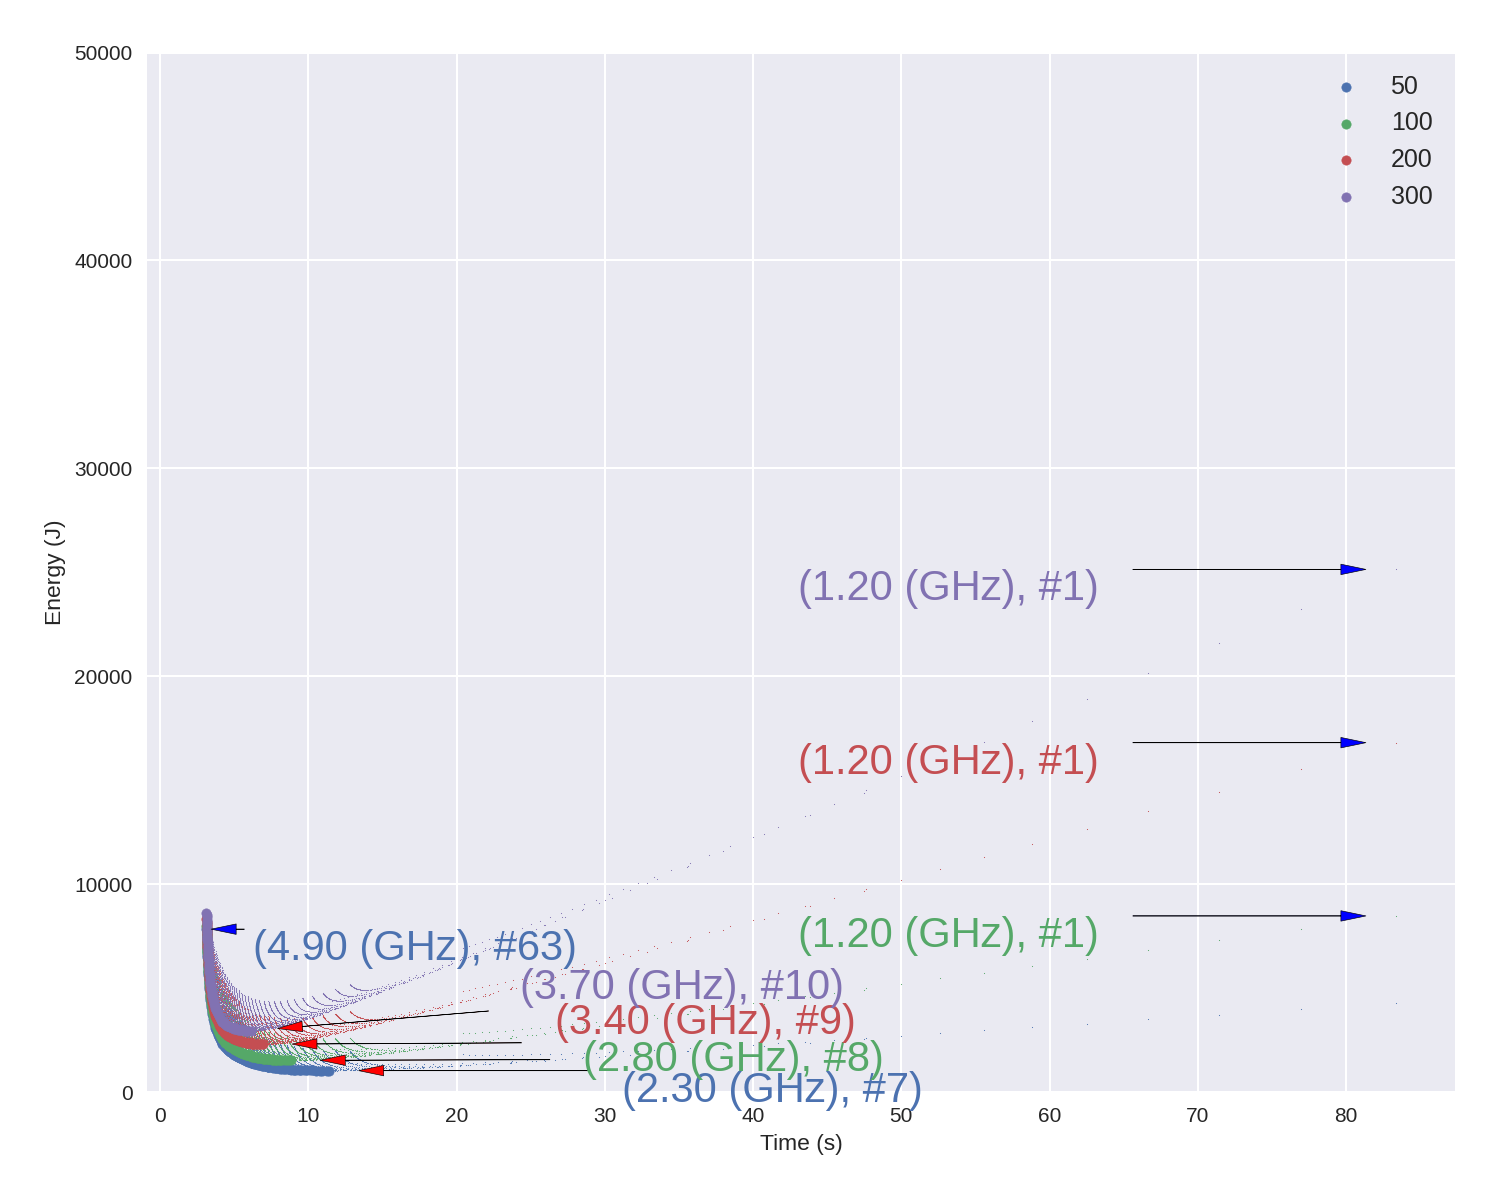
\includegraphics[width=\columnwidth]{models/figures/analisys/pareto_static_high.png}

	\caption{Pareto static energy}

	\label{fig:pareto_static_h}

\end{figure}



\begin{figure}

	\centering

	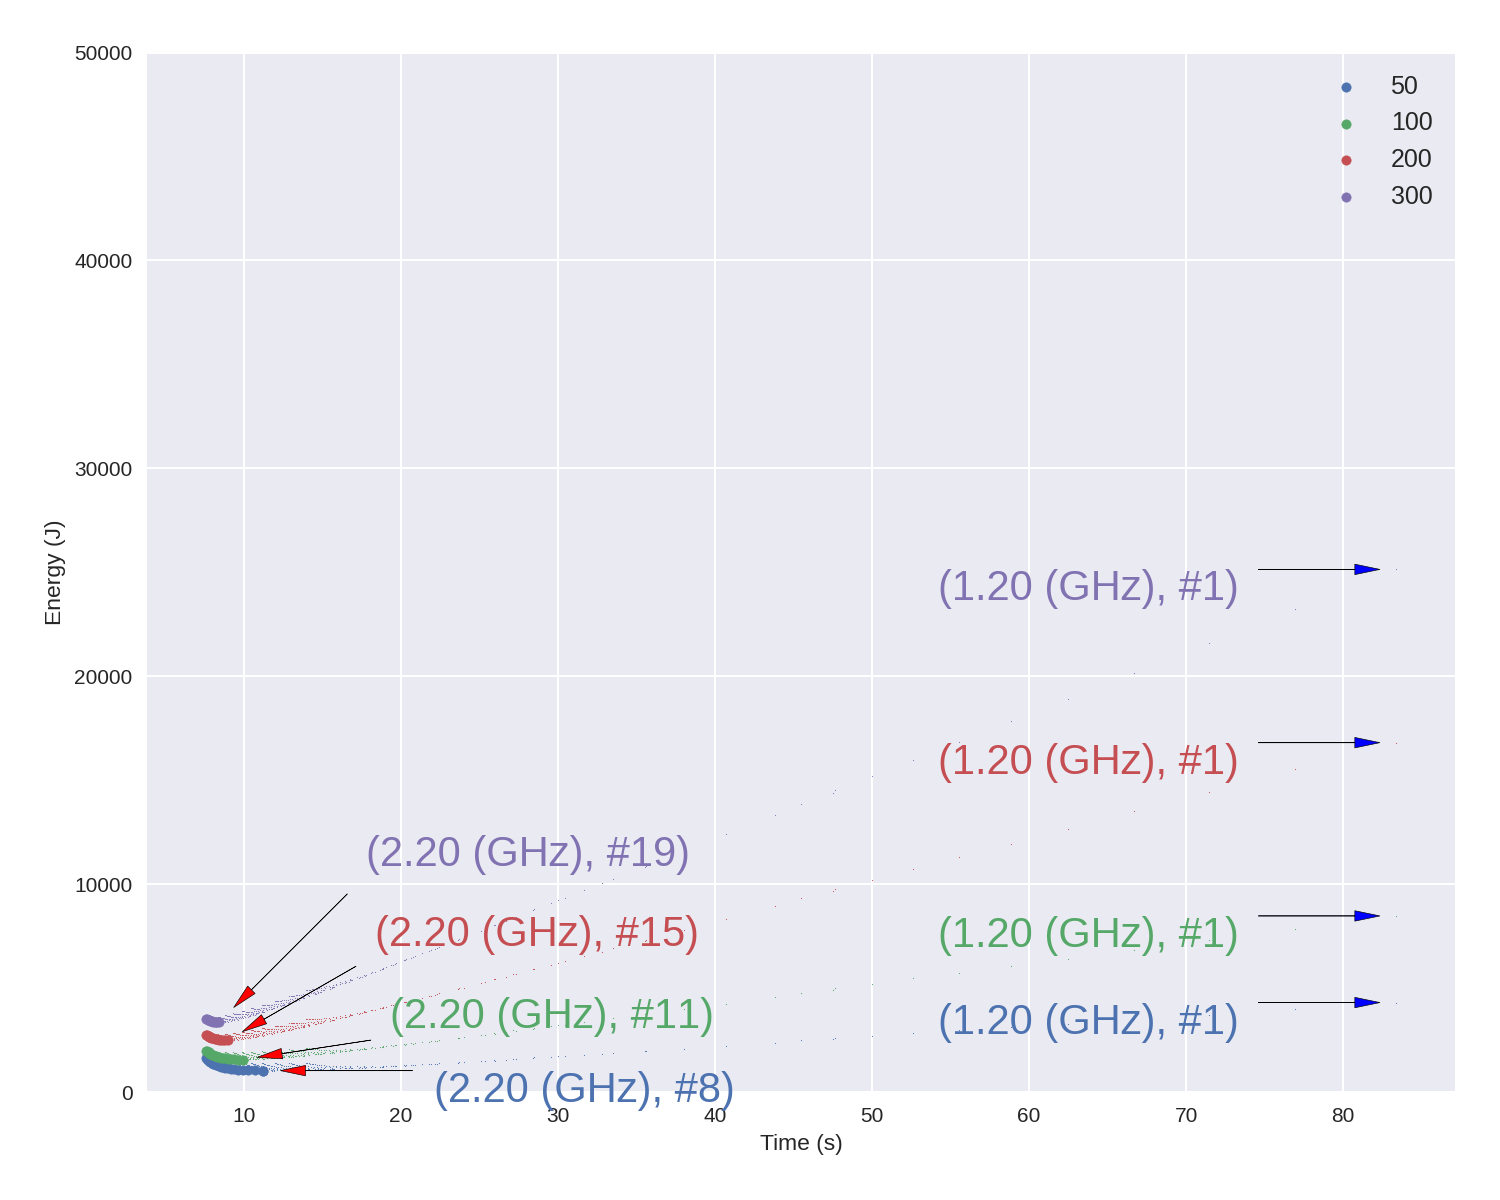
\includegraphics[width=\columnwidth]{models/figures/analisys/pareto_static_low.png}

	\caption{Pareto static energy}

	\label{fig:pareto_static_l}

\end{figure}



\begin{figure}

	\centering

	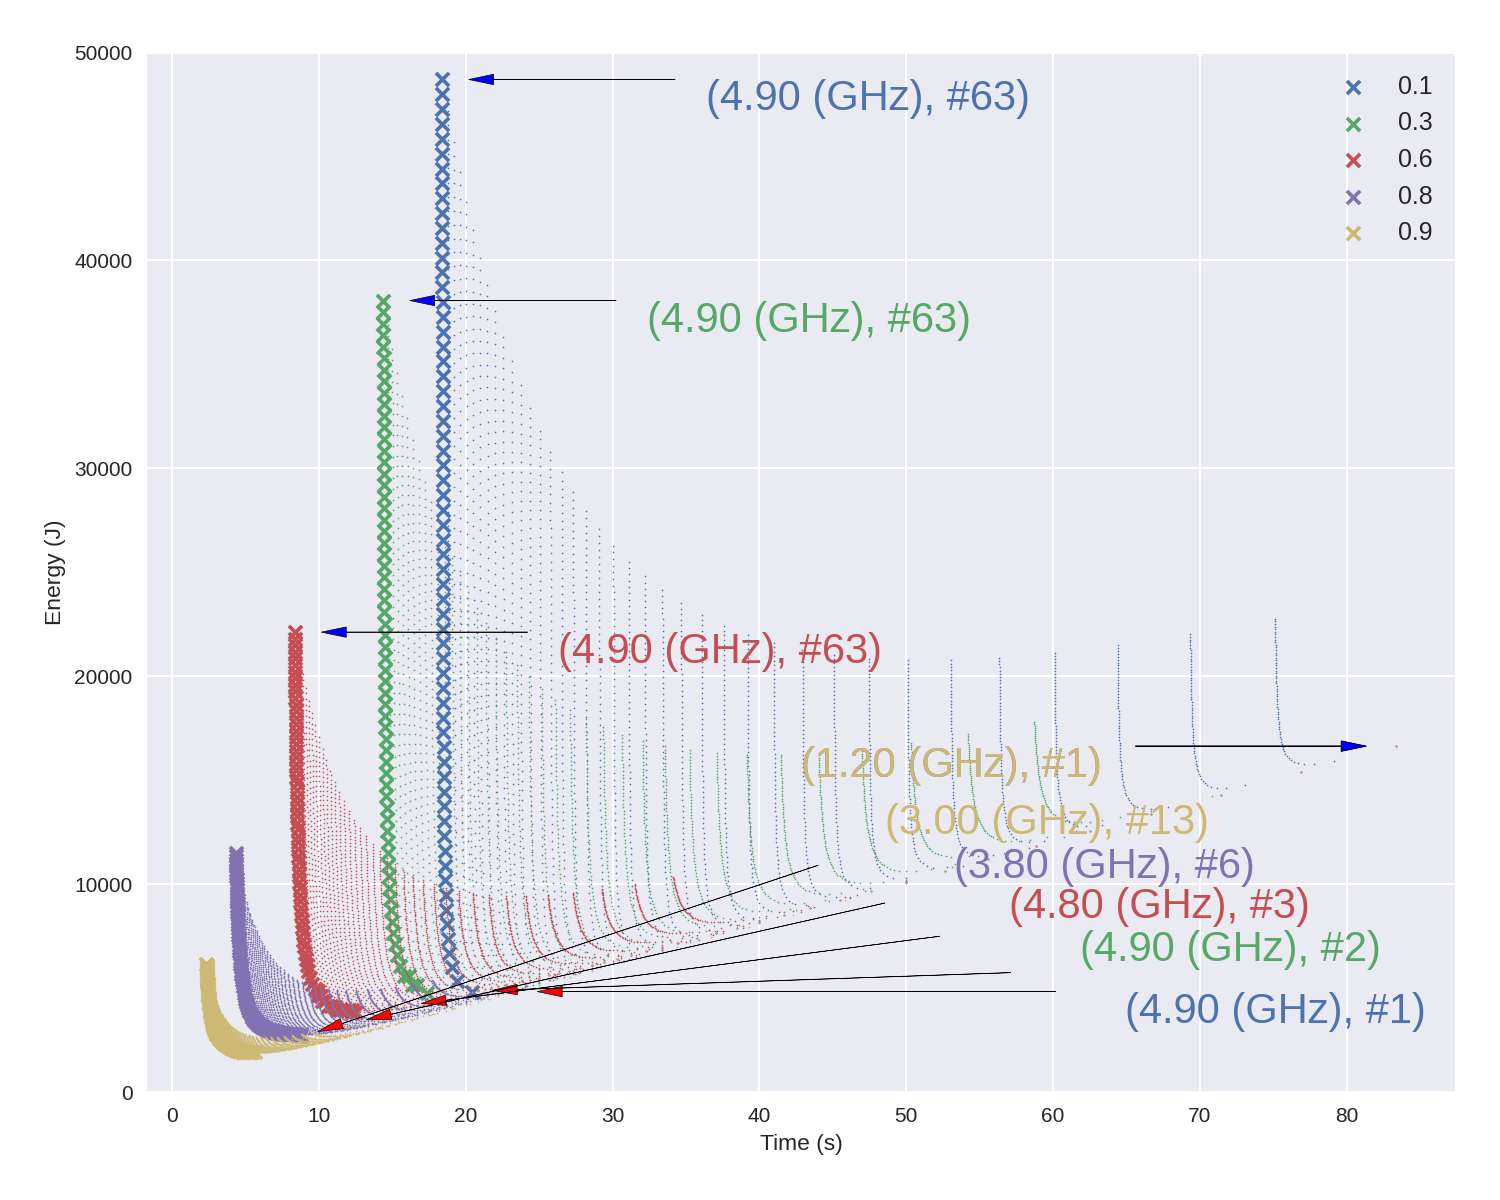
\includegraphics[width=\columnwidth]{models/figures/analisys/pareto_w_high.png}

	\caption{Pareto w energy}

	\label{fig:pareto_w_h}

\end{figure}


\begin{figure}

	\centering

	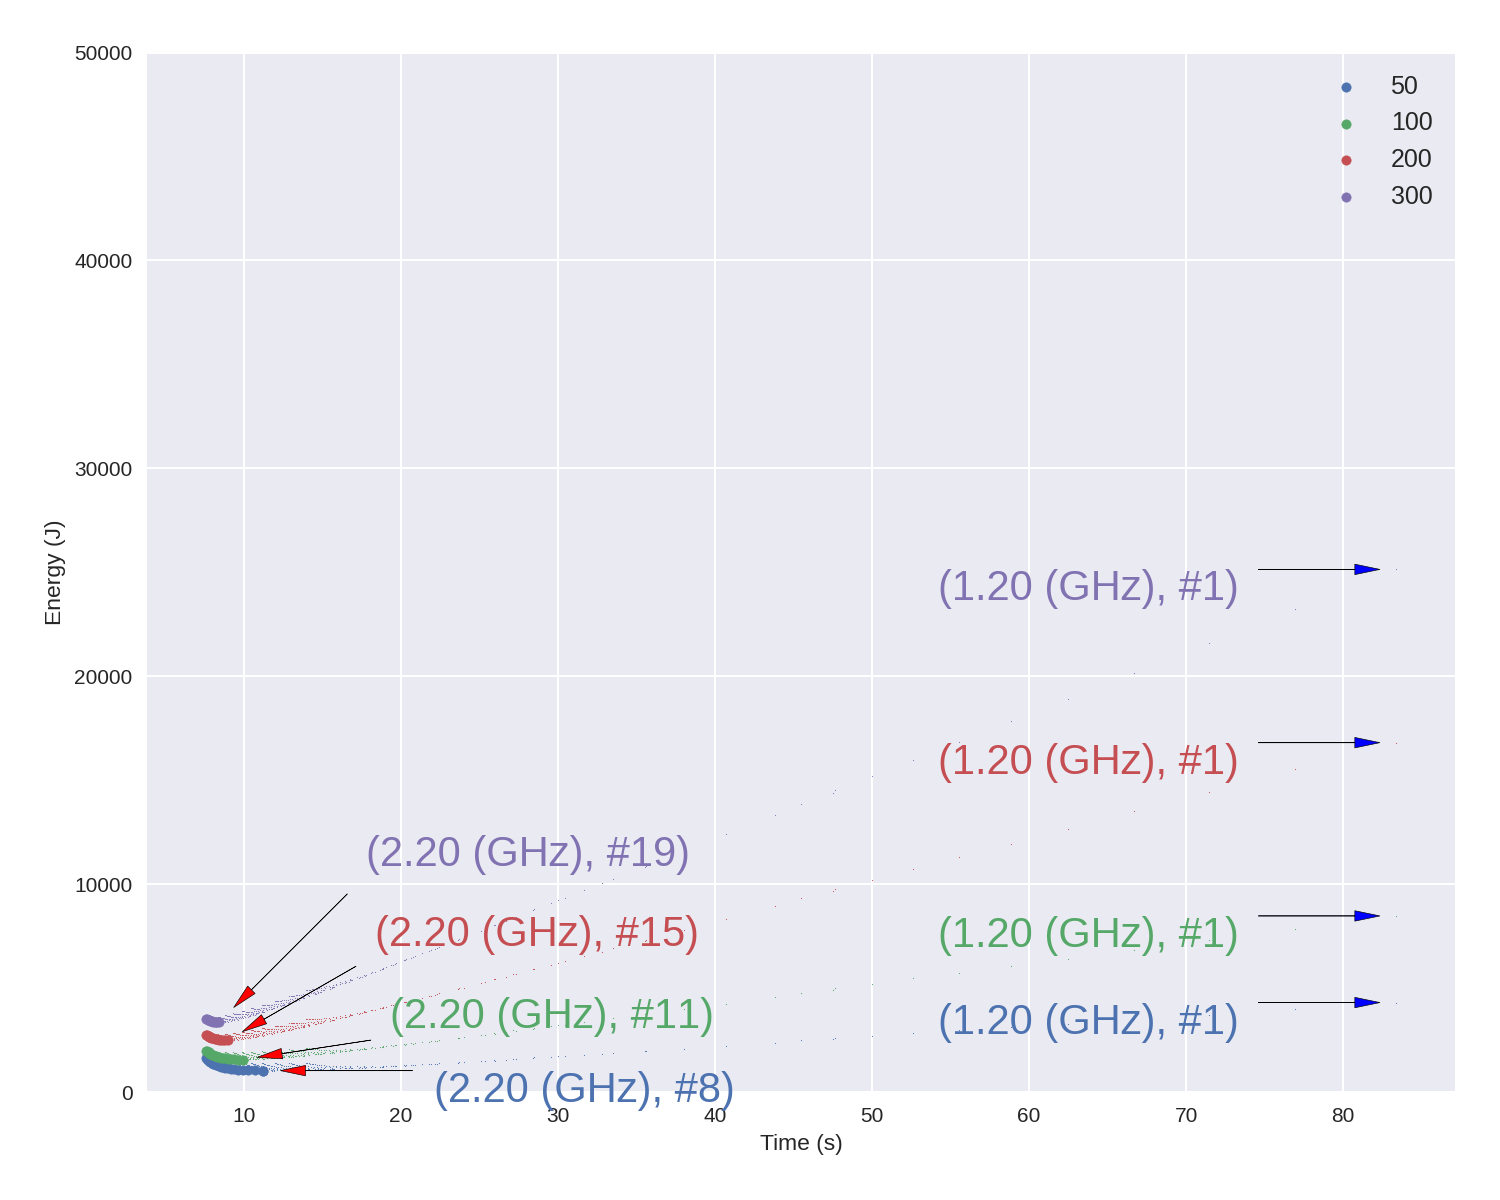
\includegraphics[width=\columnwidth]{models/figures/analisys/pareto_static_low.png}

	\caption{Pareto w energy}

	\label{fig:pareto_w_l}

\end{figure}


\subsection{Optimization under constraints}


\subsection{Gradient and Countorns}


\begin{figure}[H]

	\centering

	\begin{subfigure}[b]{0.45\textwidth}

		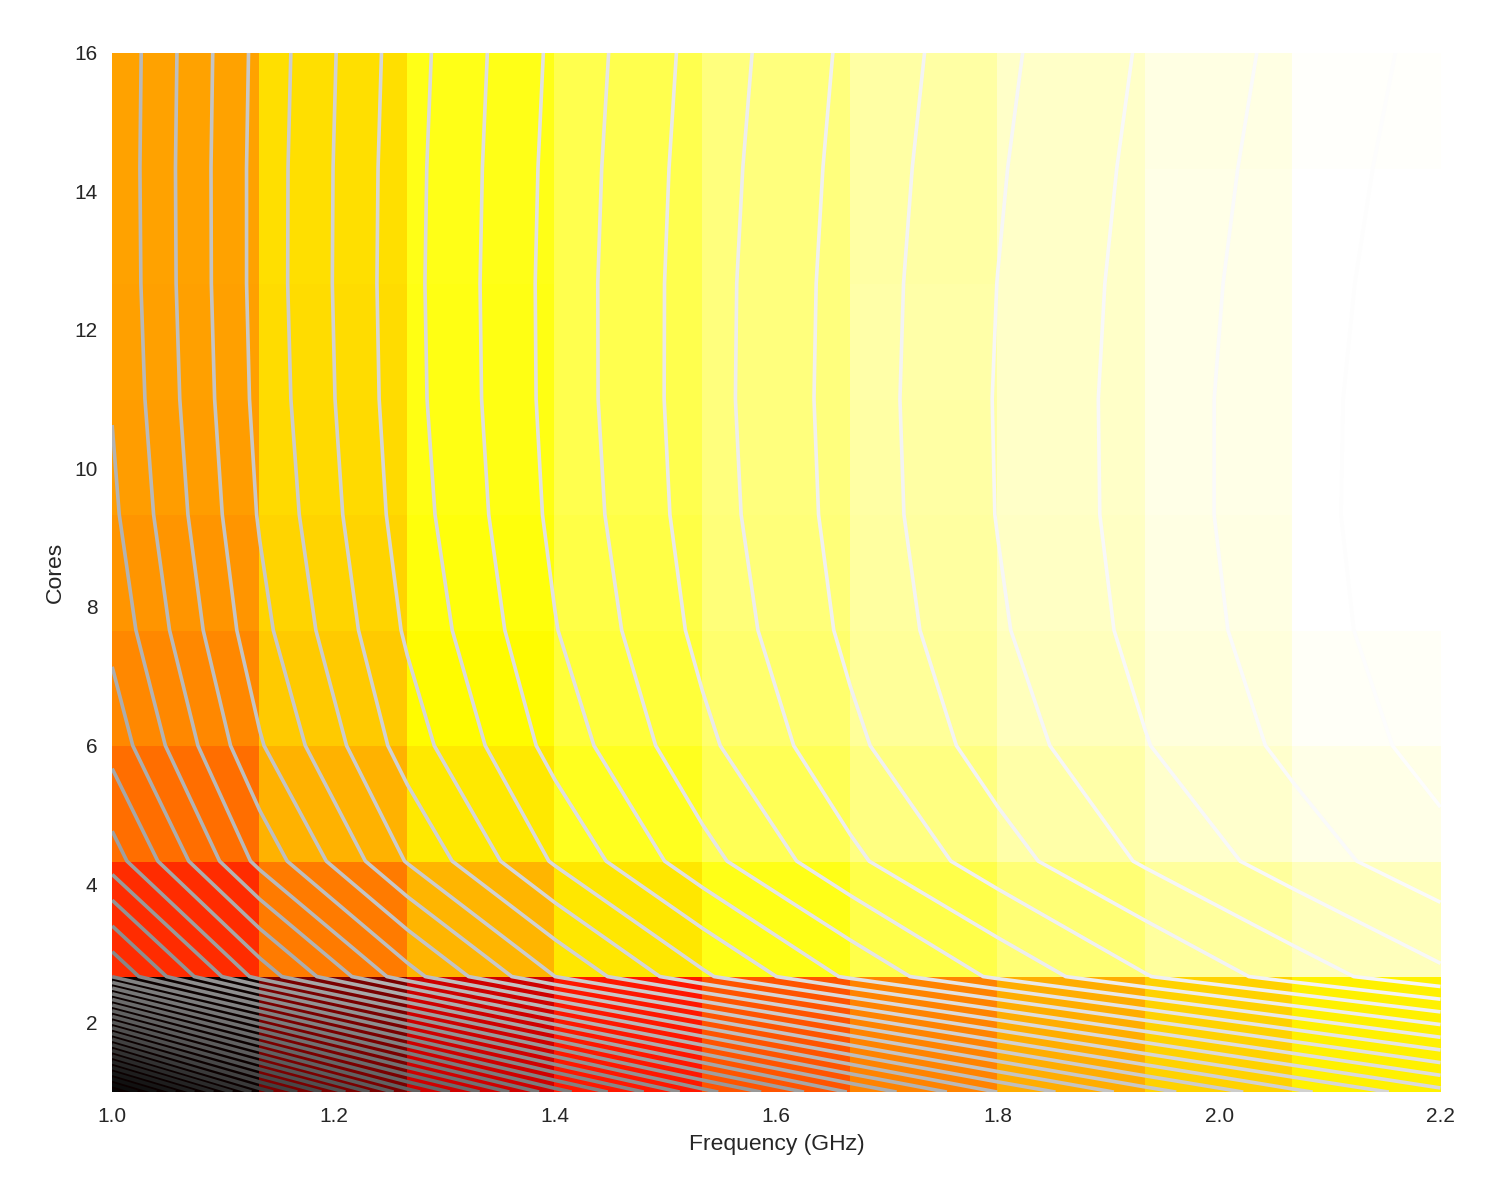
\includegraphics[width=\textwidth]{models/figures/analisys/pdyn0.png}

	\end{subfigure}

	%

	\begin{subfigure}[b]{0.45\textwidth}

		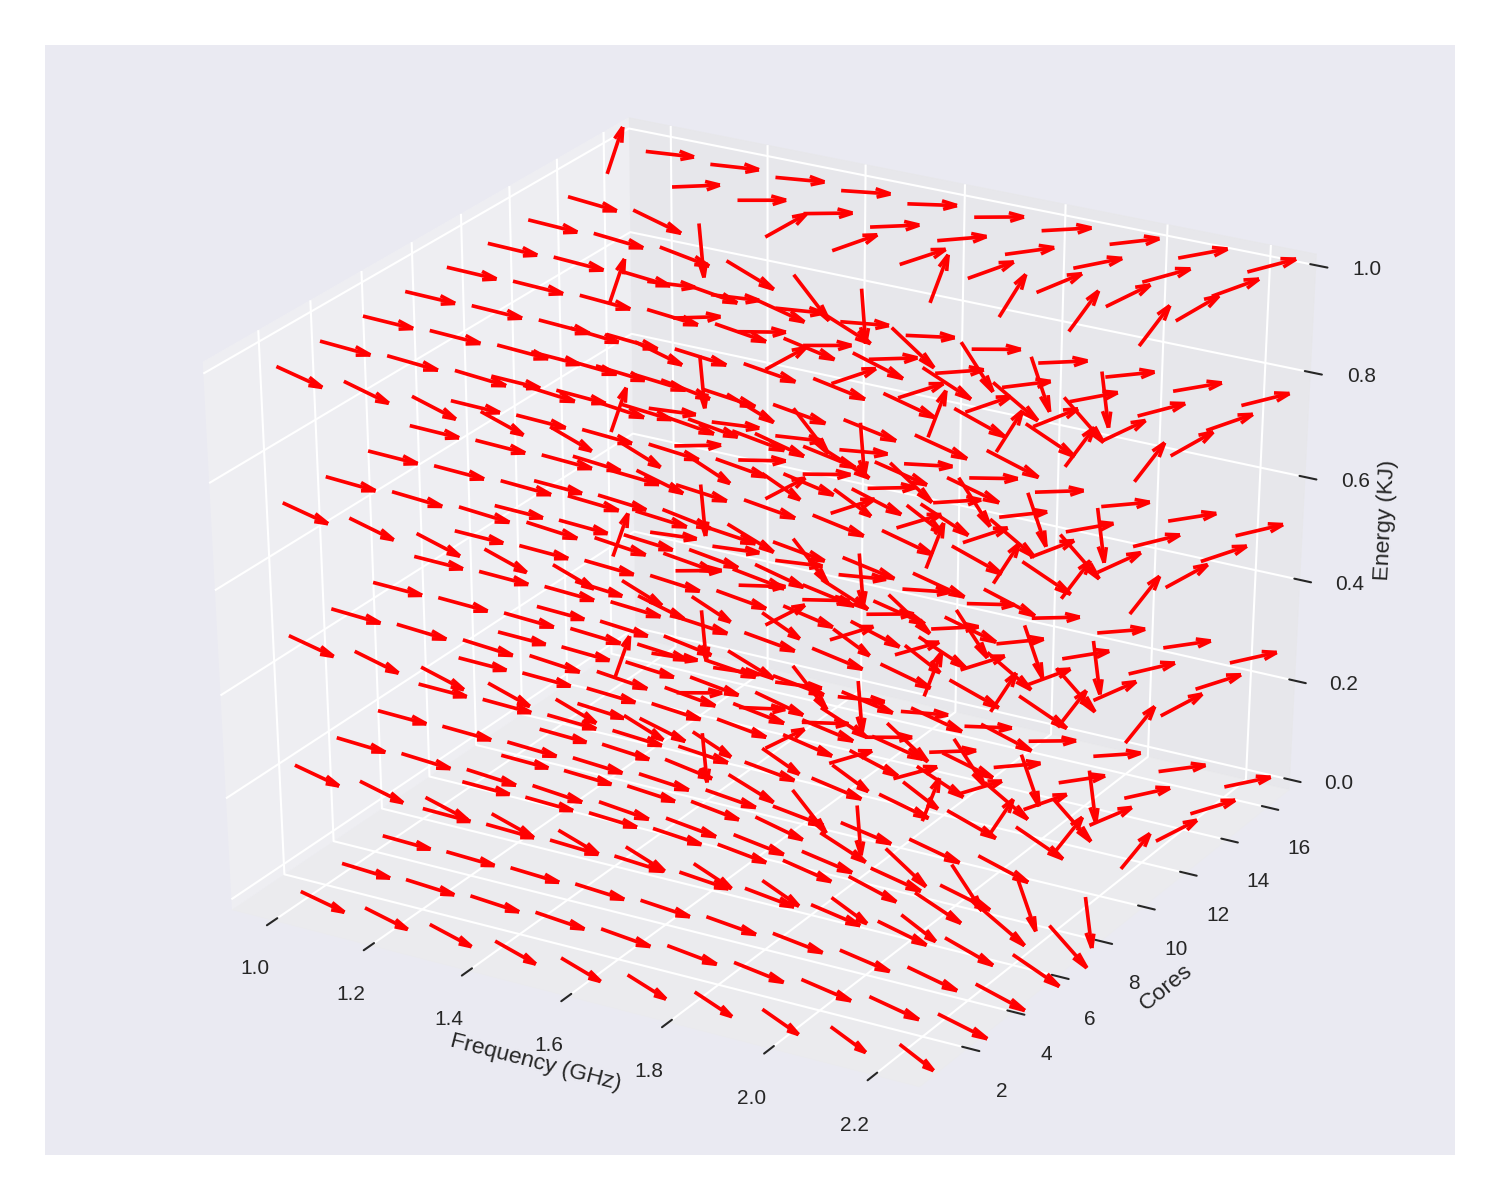
\includegraphics[width=\textwidth]{models/figures/analisys/pdyn0_3d.png}

	\end{subfigure}

\end{figure}


\begin{figure}[H]

	\centering

	\begin{subfigure}[b]{0.45\textwidth}

		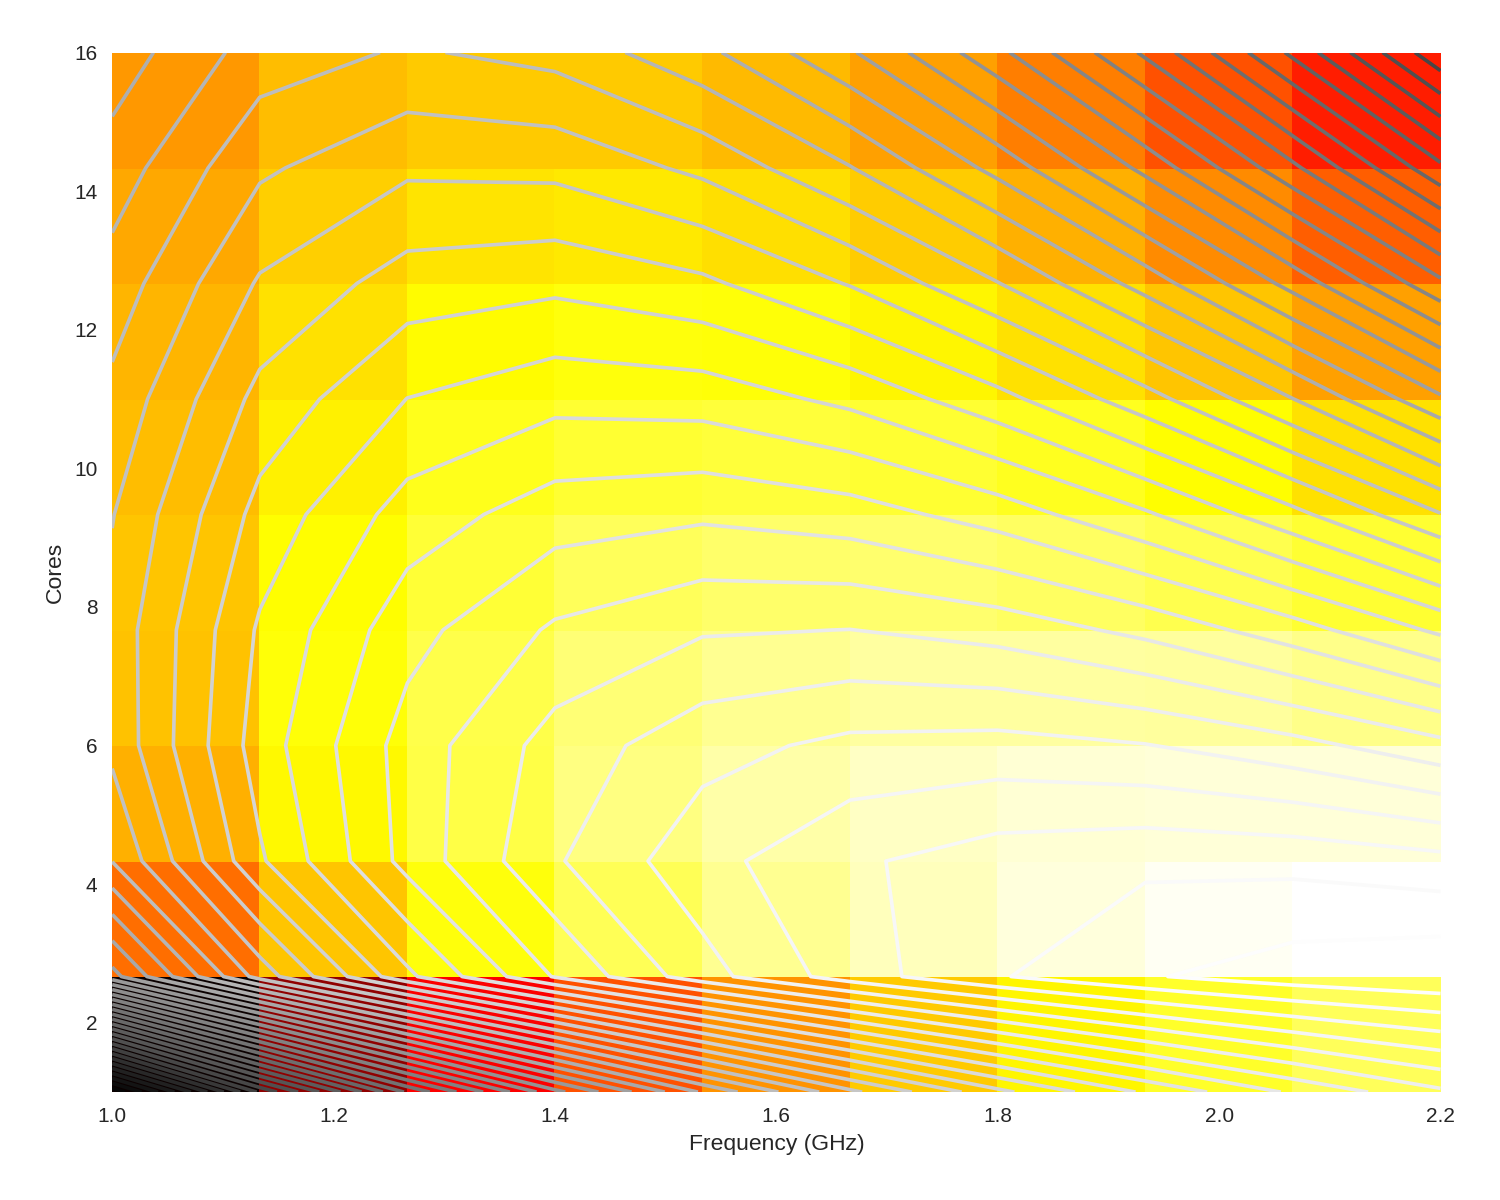
\includegraphics[width=\textwidth]{models/figures/analisys/pdyn3.png}

	\end{subfigure}

	%

	\begin{subfigure}[b]{0.45\textwidth}

		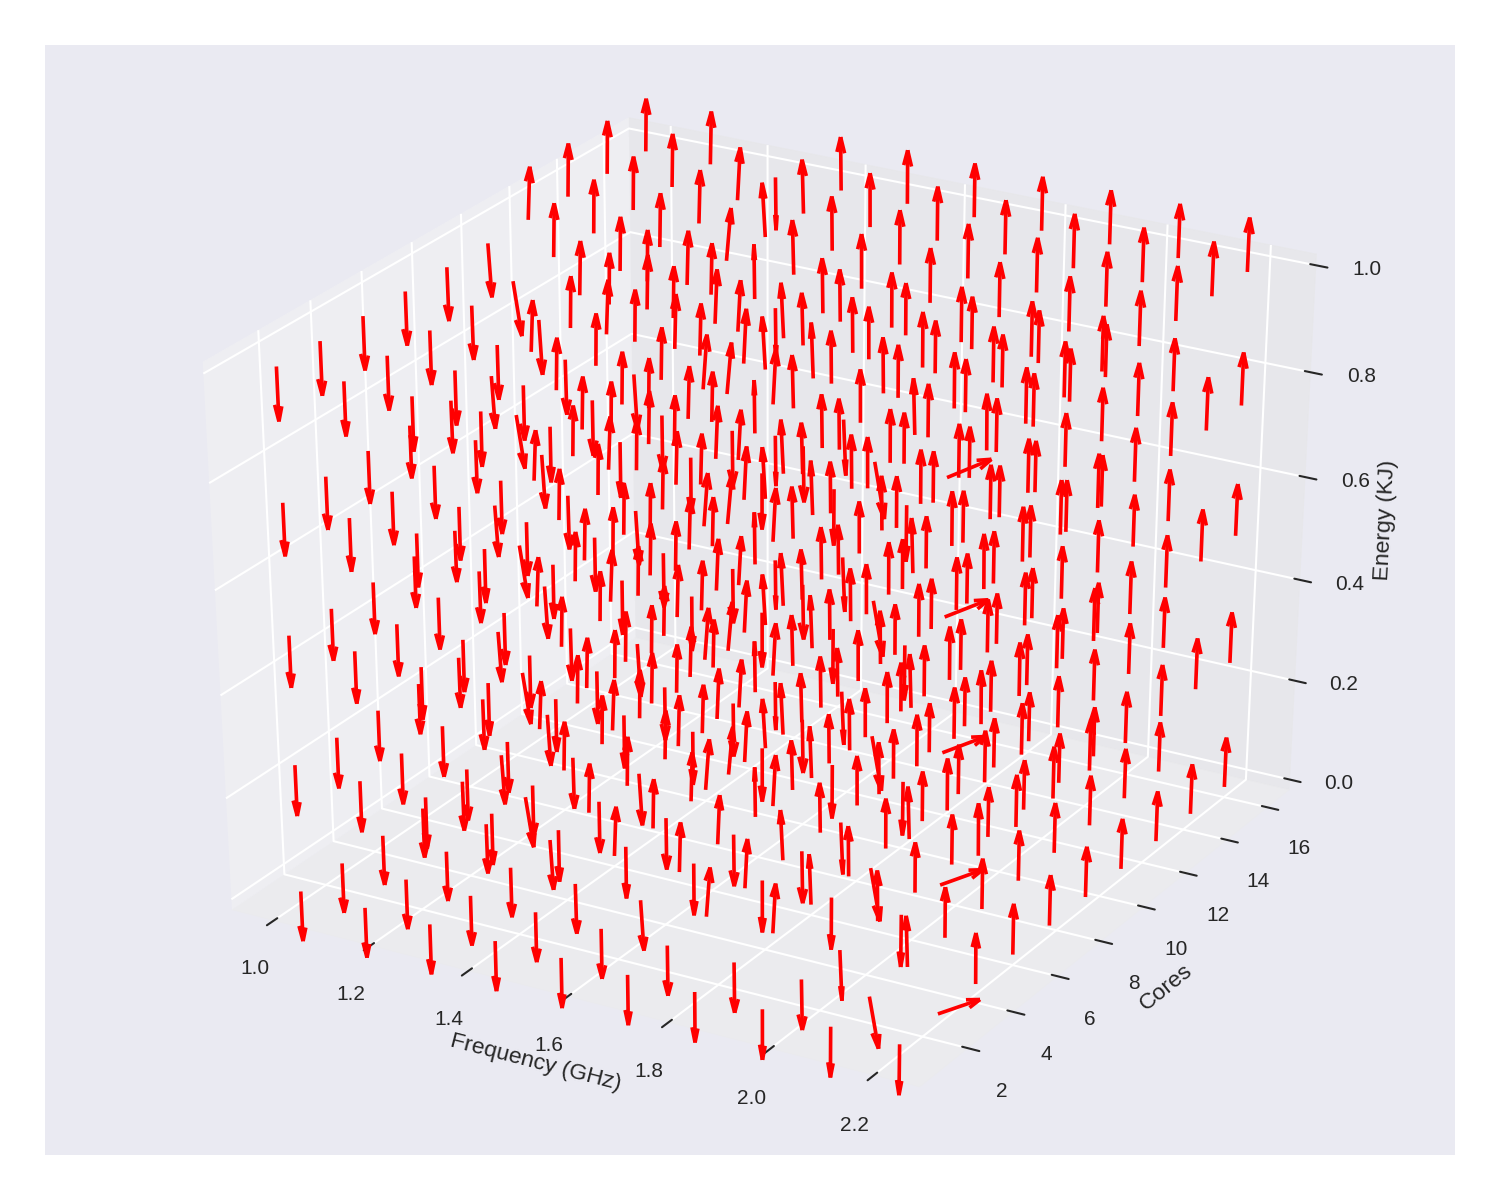
\includegraphics[width=\textwidth]{models/figures/analisys/pdyn3_3d.png}

	\end{subfigure}

\end{figure}


\begin{figure}[H]

	\centering

	\begin{subfigure}[b]{0.45\textwidth}

		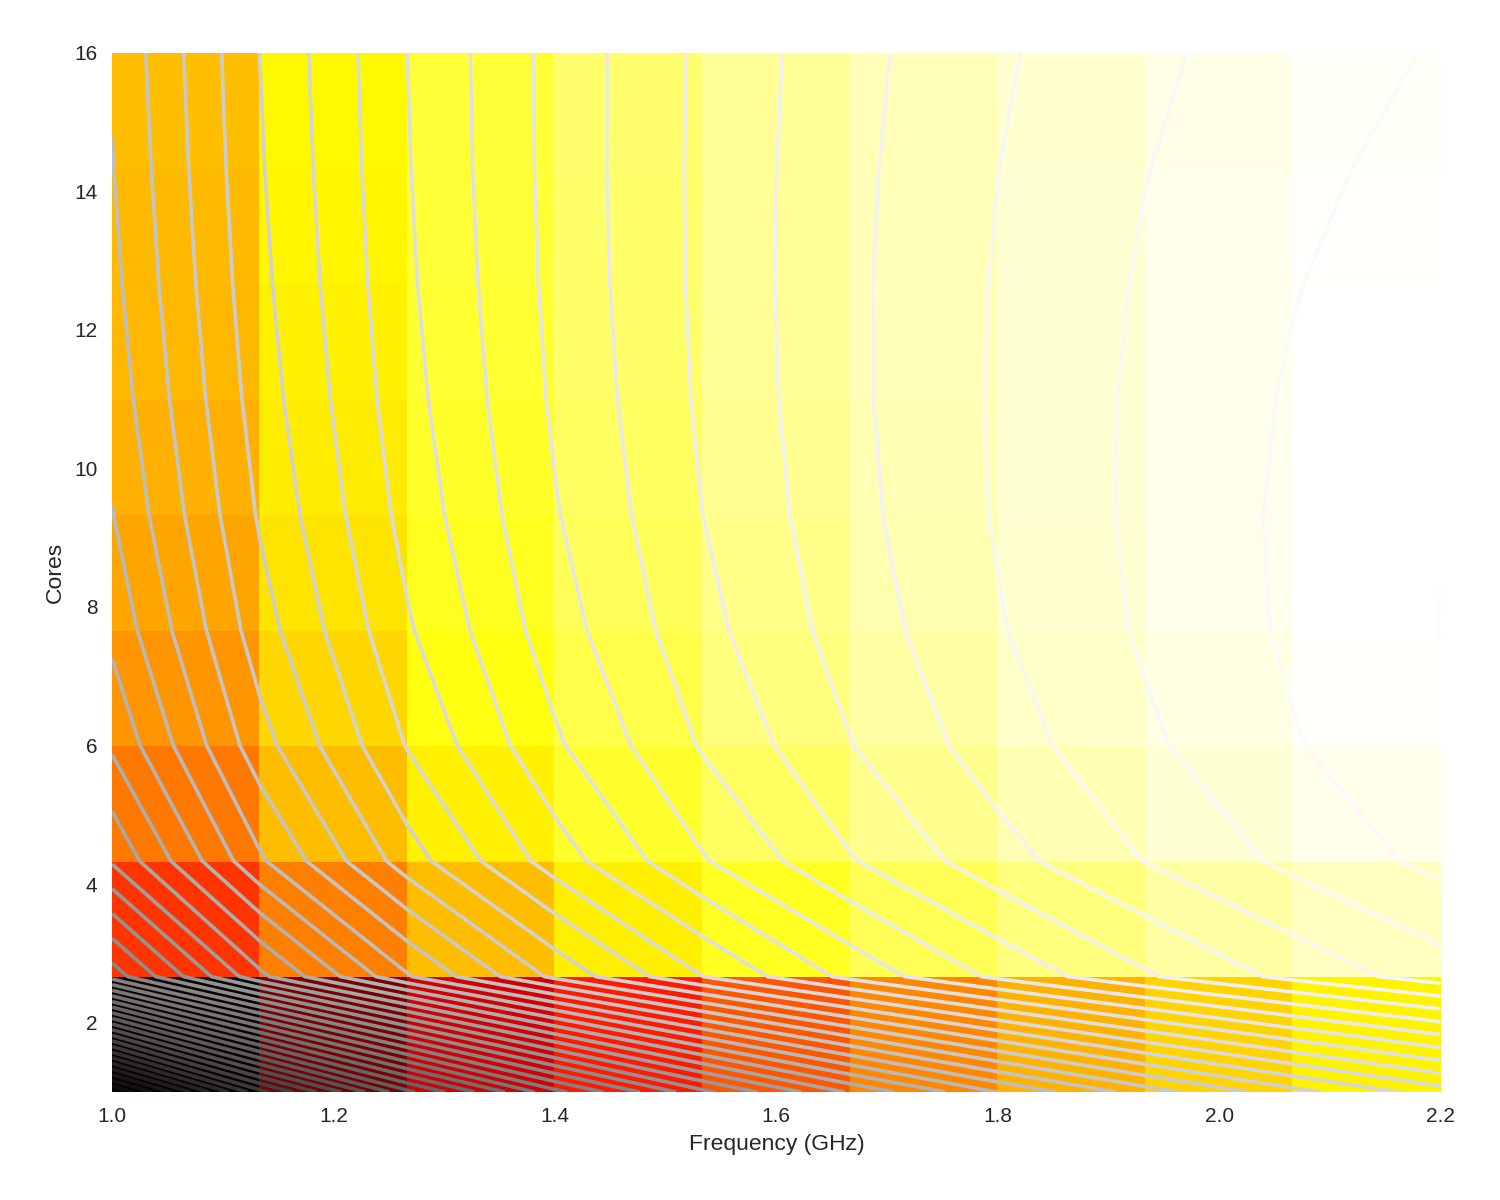
\includegraphics[width=\textwidth]{models/figures/analisys/pleak0.png}

	\end{subfigure}

	%

	\begin{subfigure}[b]{0.45\textwidth}

		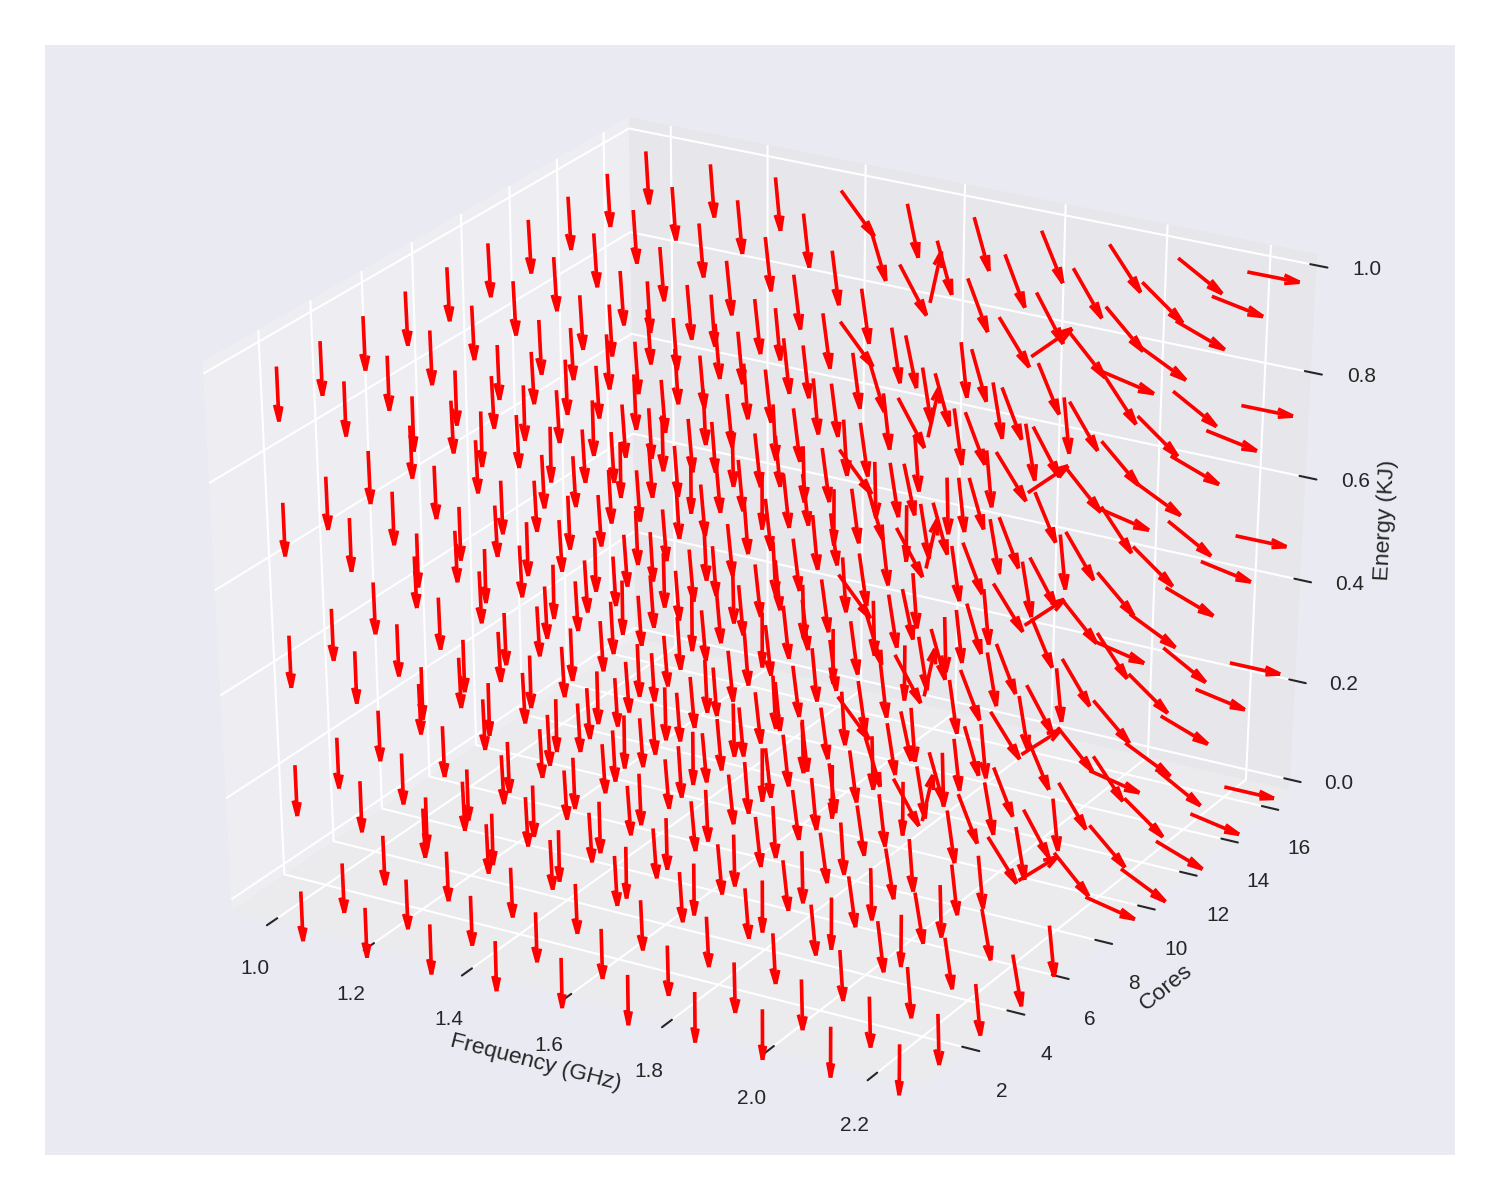
\includegraphics[width=\textwidth]{models/figures/analisys/pleak0_3d.png}

	\end{subfigure}

\end{figure}


\begin{figure}[H]

	\centering

	\begin{subfigure}[b]{0.45\textwidth}

		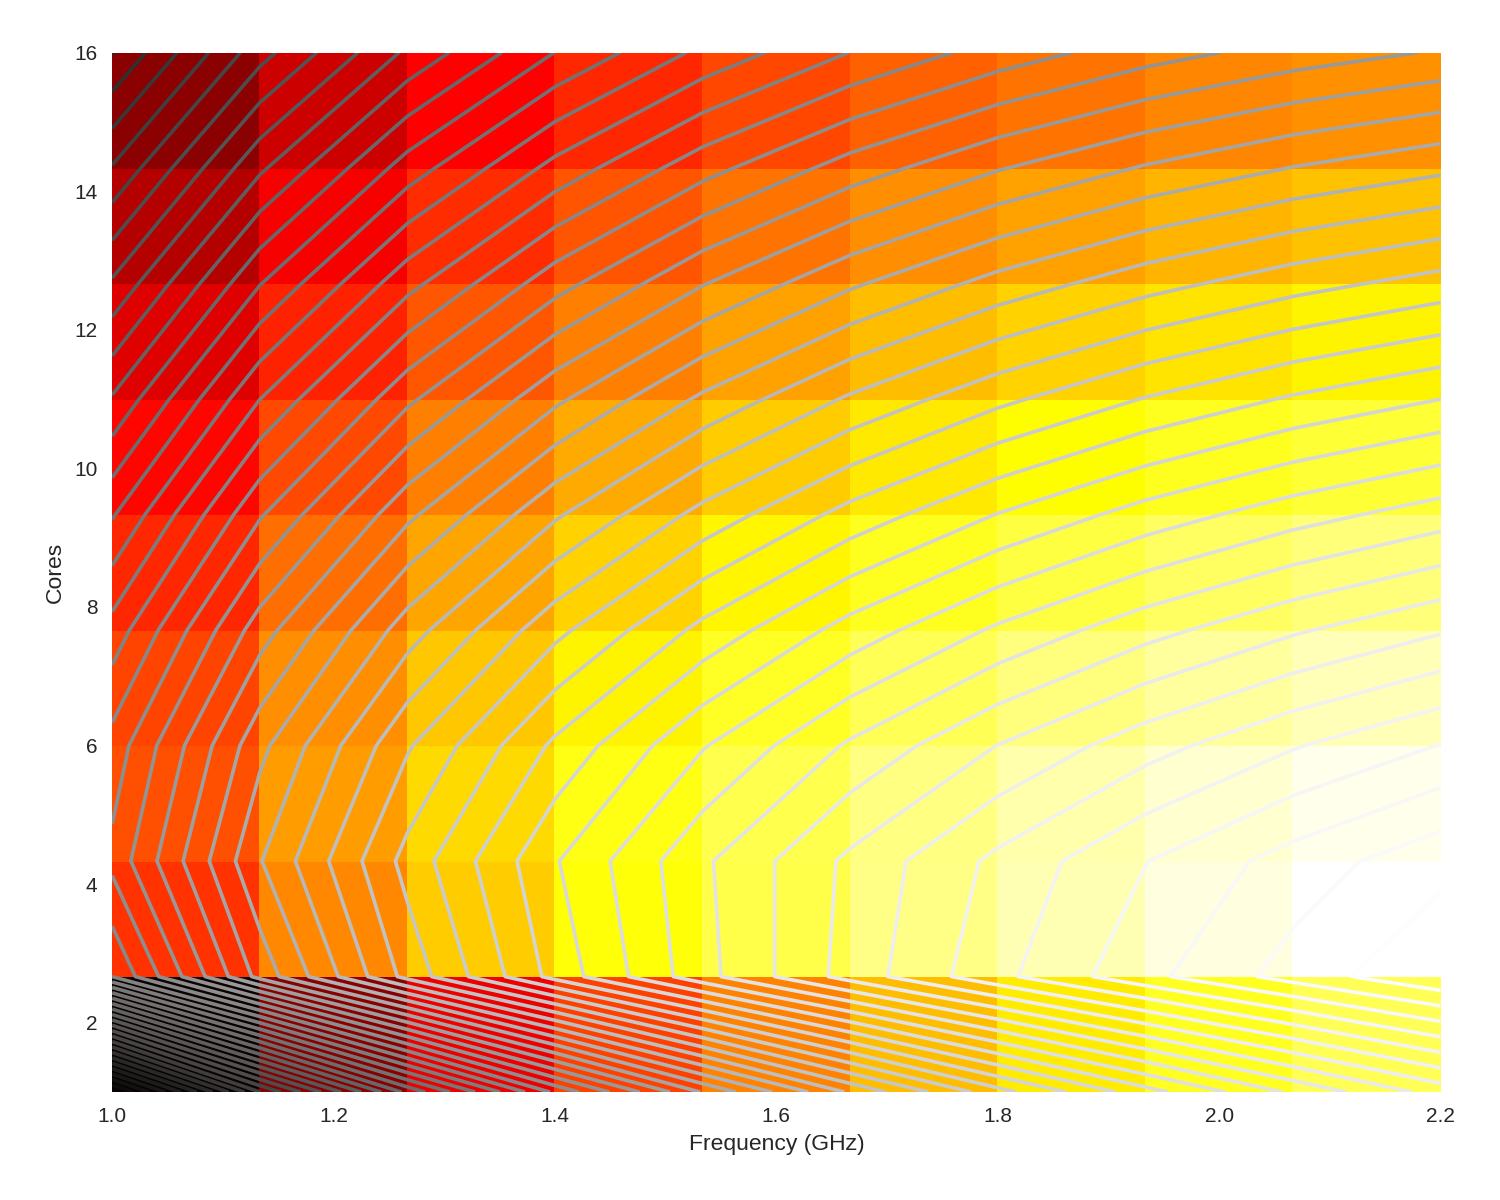
\includegraphics[width=\textwidth]{models/figures/analisys/pleak10.png}

	\end{subfigure}

	%

	\begin{subfigure}[b]{0.45\textwidth}

		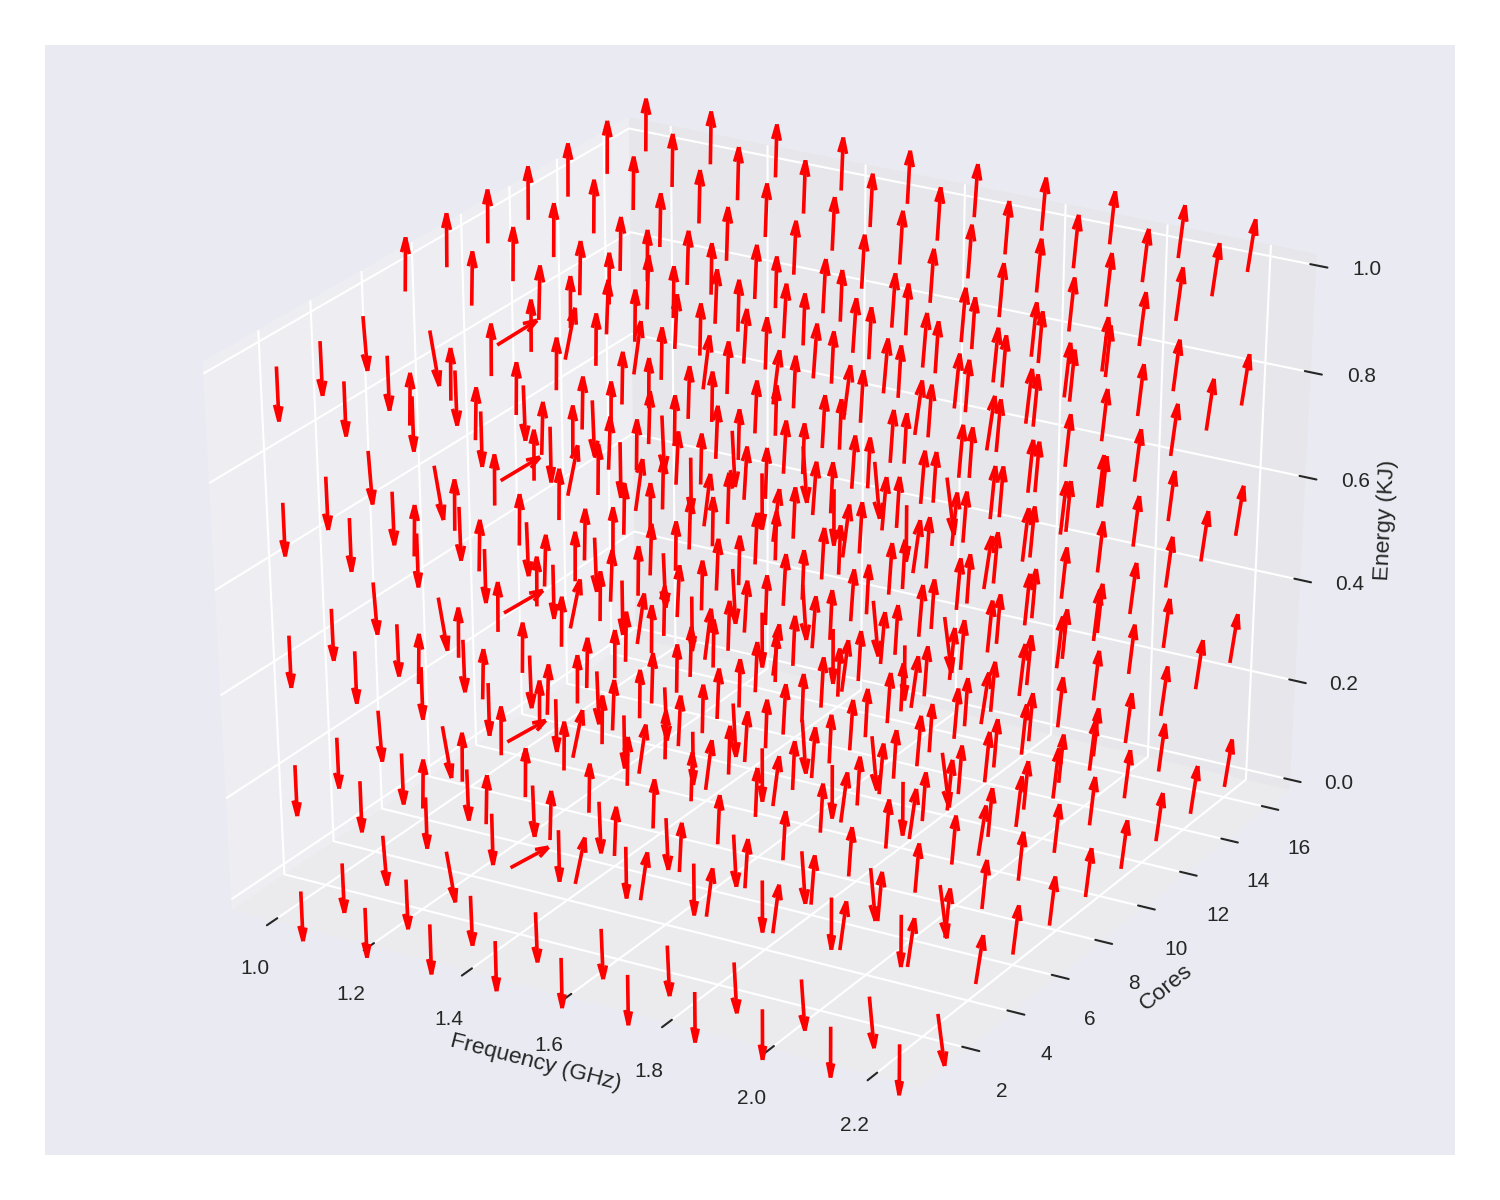
\includegraphics[width=\textwidth]{models/figures/analisys/pleak10_3d.png}

	\end{subfigure}

\end{figure}


\begin{figure}[H]

	\centering

	\begin{subfigure}[b]{0.45\textwidth}

		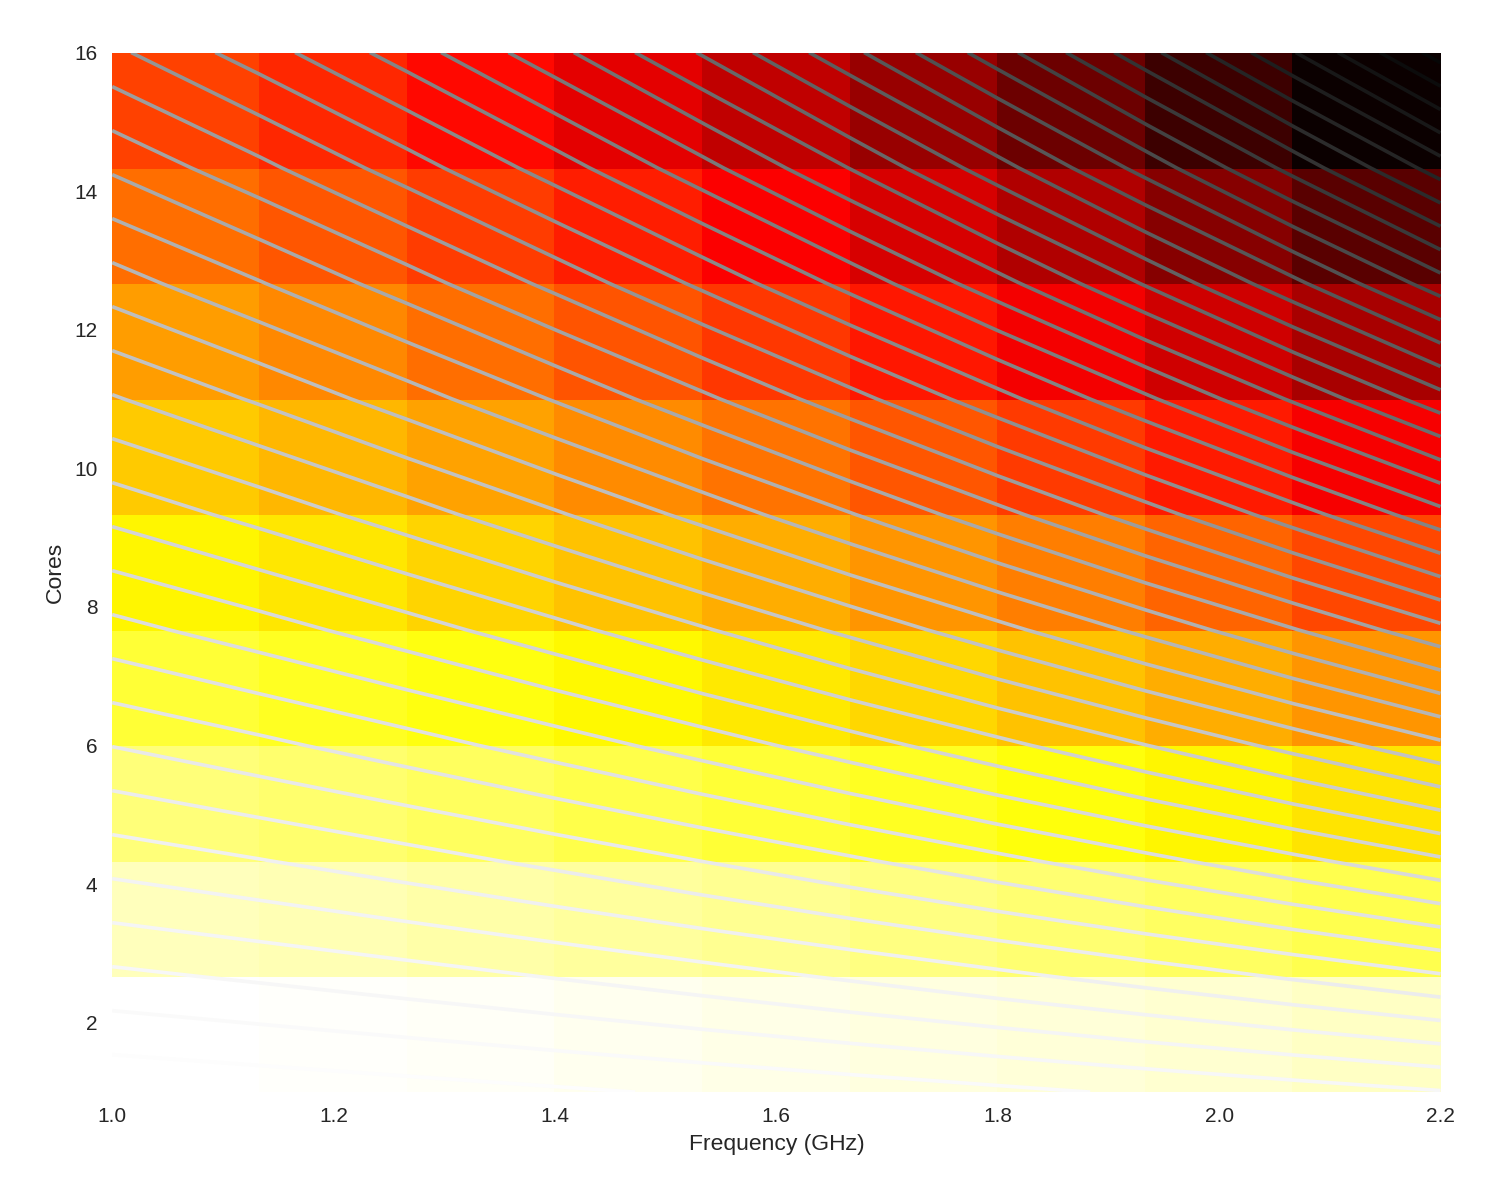
\includegraphics[width=\textwidth]{models/figures/analisys/pstatic0.png}

	\end{subfigure}

	%

	\begin{subfigure}[b]{0.45\textwidth}

		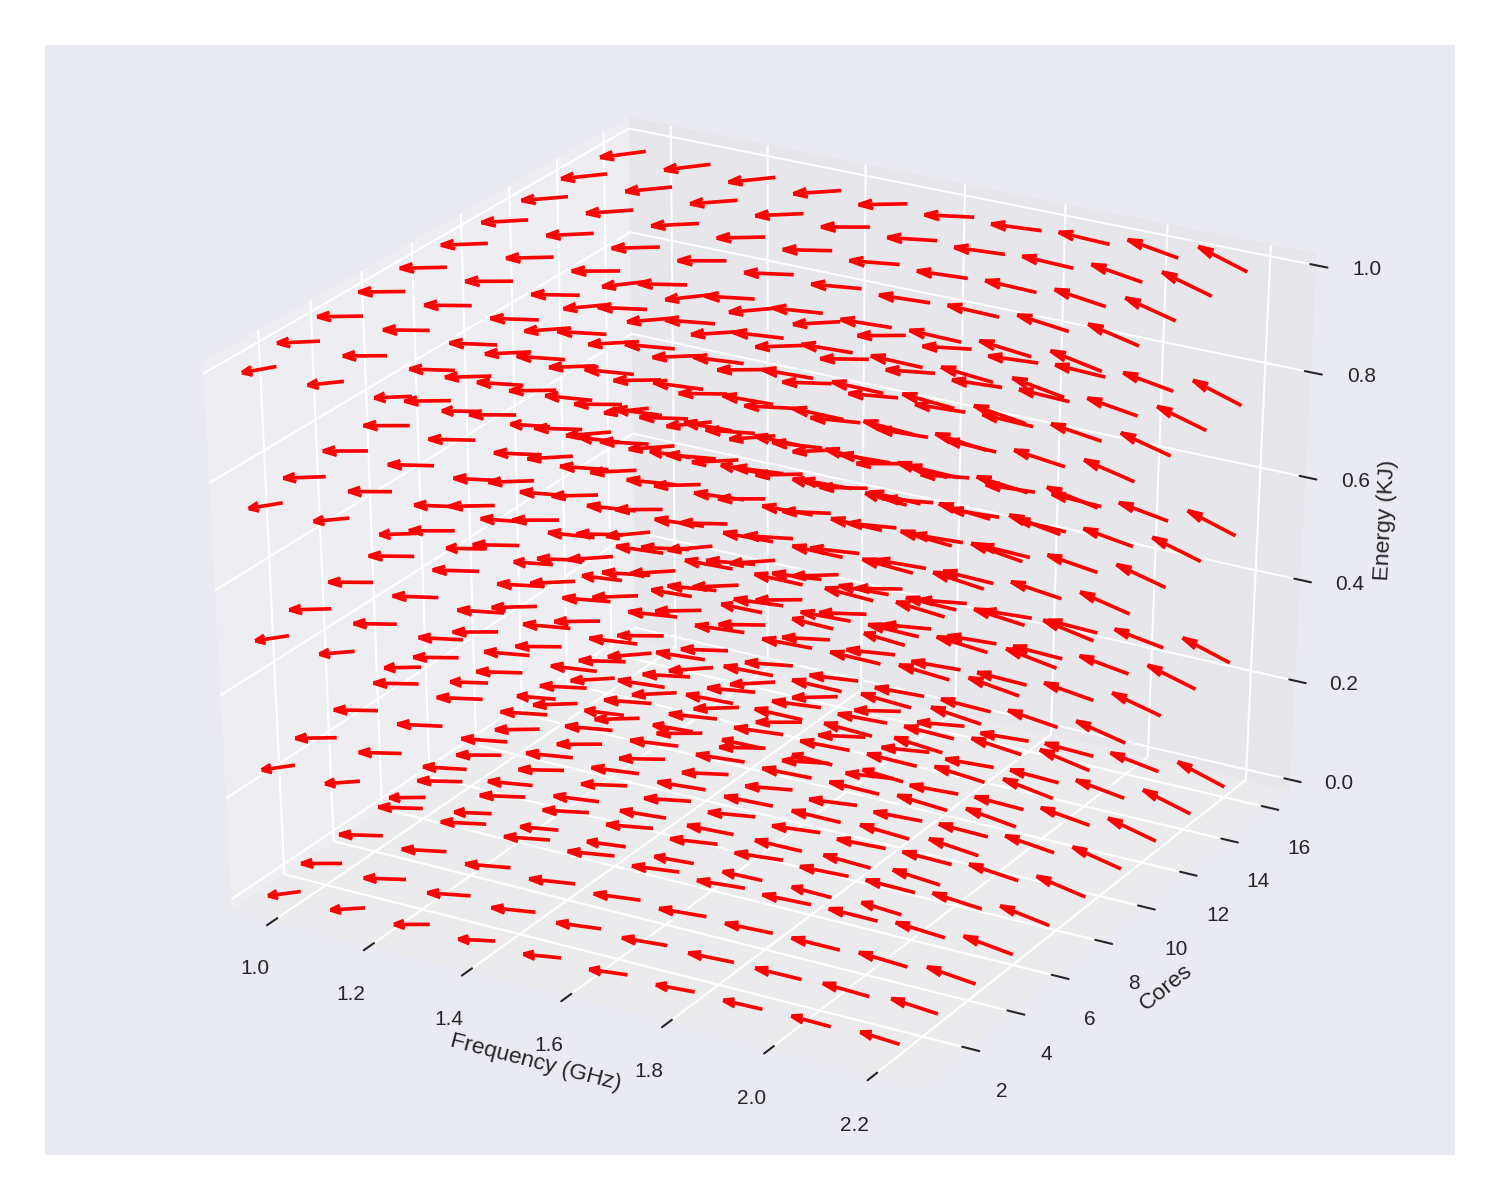
\includegraphics[width=\textwidth]{models/figures/analisys/pstatic0_3d.png}

	\end{subfigure}

\end{figure}


\begin{figure}[H]

	\centering

	\begin{subfigure}[b]{0.45\textwidth}

		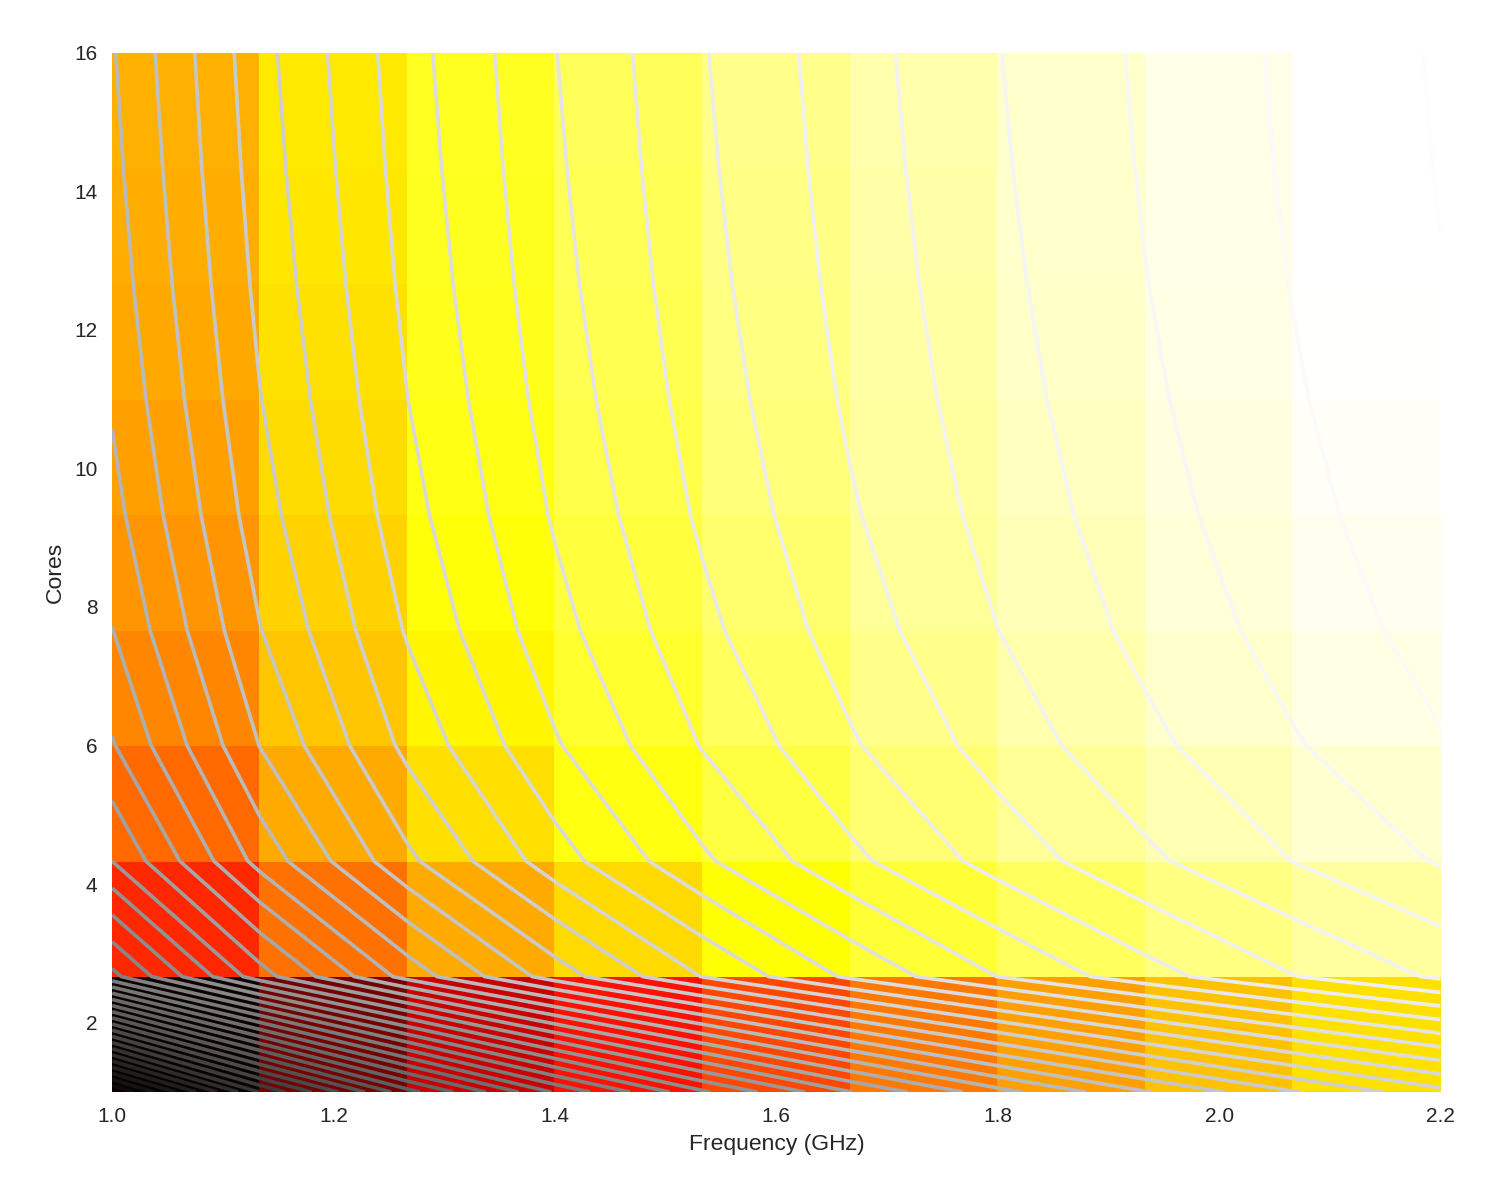
\includegraphics[width=\textwidth]{models/figures/analisys/pstatic3000.png}

	\end{subfigure}

	%

	\begin{subfigure}[b]{0.45\textwidth}

		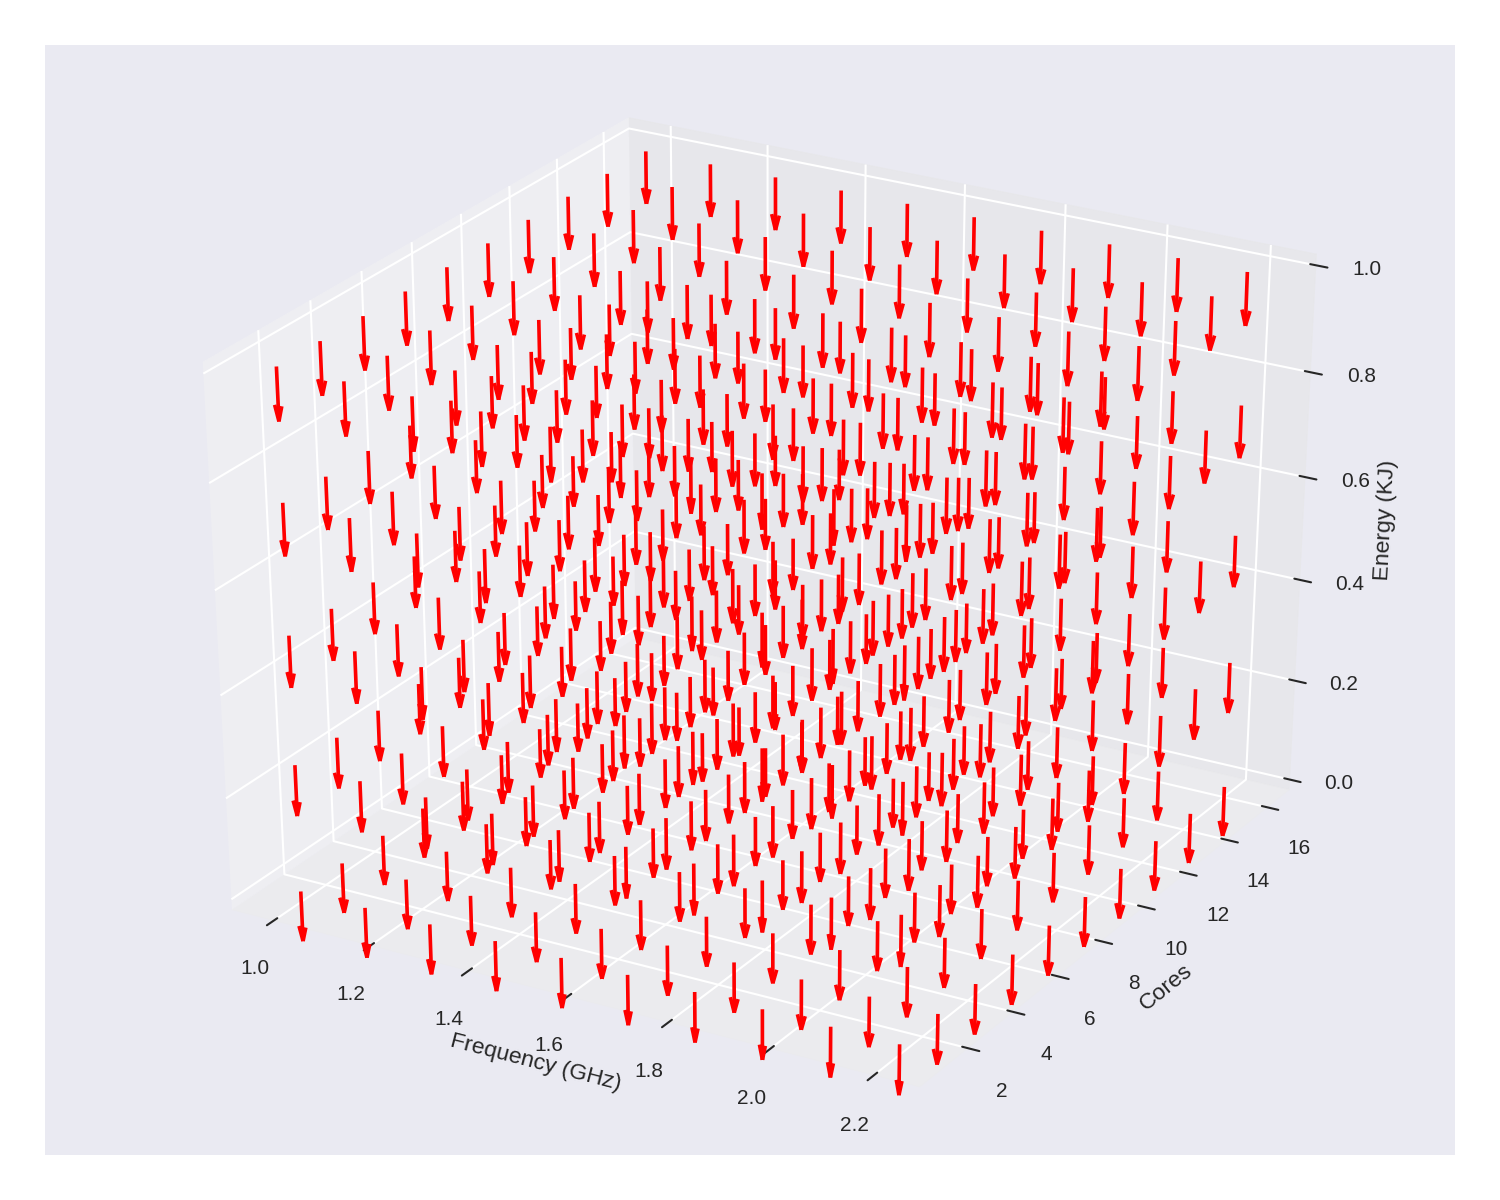
\includegraphics[width=\textwidth]{models/figures/analisys/pstatic3000_3d.png}

	\end{subfigure}

\end{figure}


\begin{figure}[H]

	\centering

	\begin{subfigure}[b]{0.45\textwidth}

		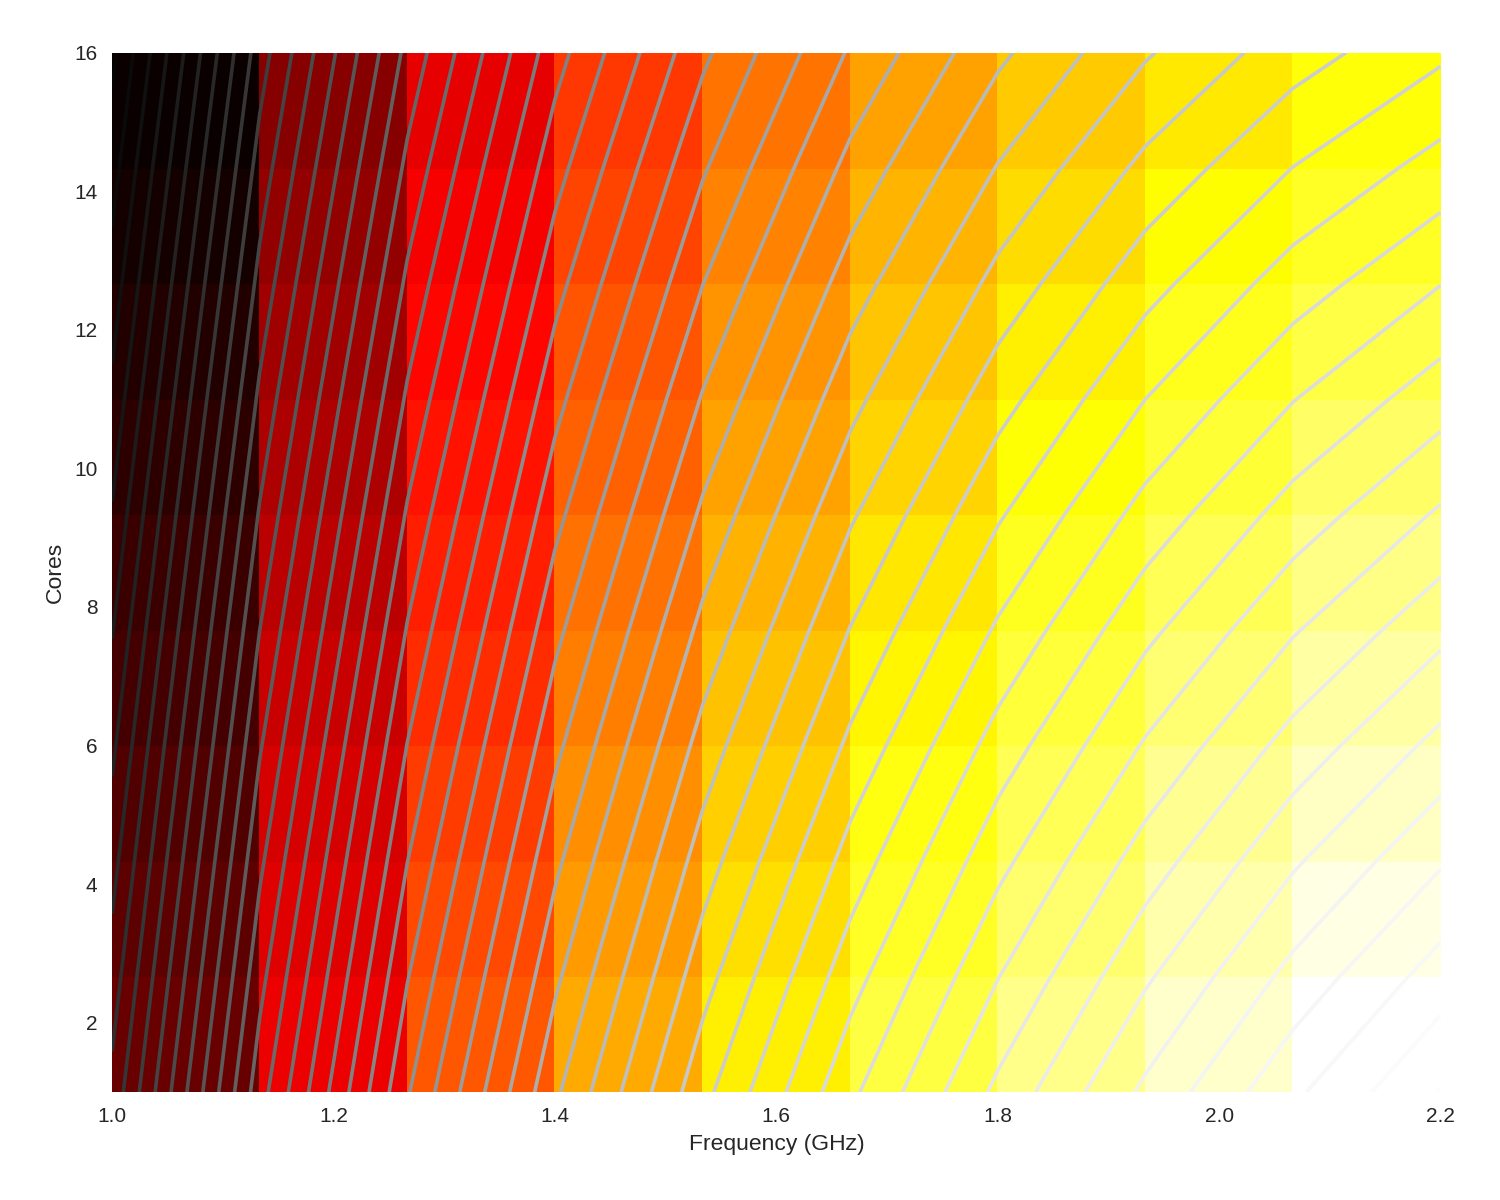
\includegraphics[width=\textwidth]{models/figures/analisys/w0.png}

	\end{subfigure}

	%

	\begin{subfigure}[b]{0.45\textwidth}

		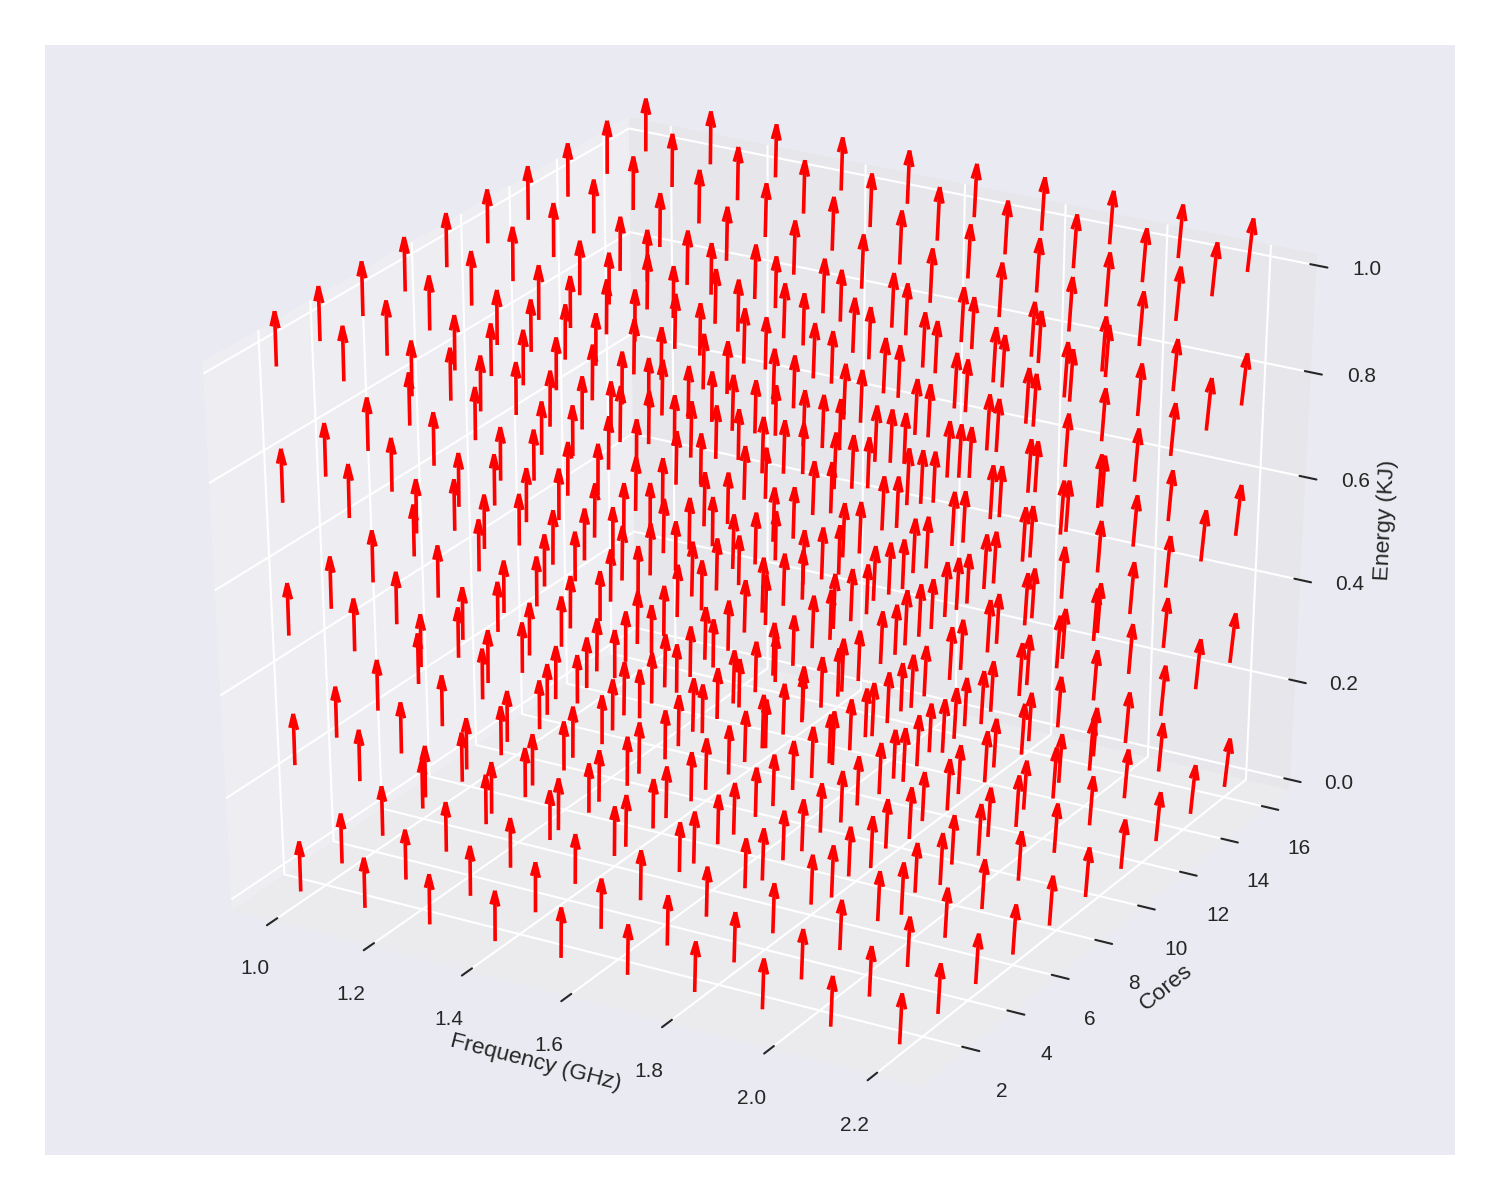
\includegraphics[width=\textwidth]{models/figures/analisys/w0_3d.png}

	\end{subfigure}

\end{figure}


\begin{figure}[H]

	\centering

	\begin{subfigure}[b]{0.45\textwidth}

		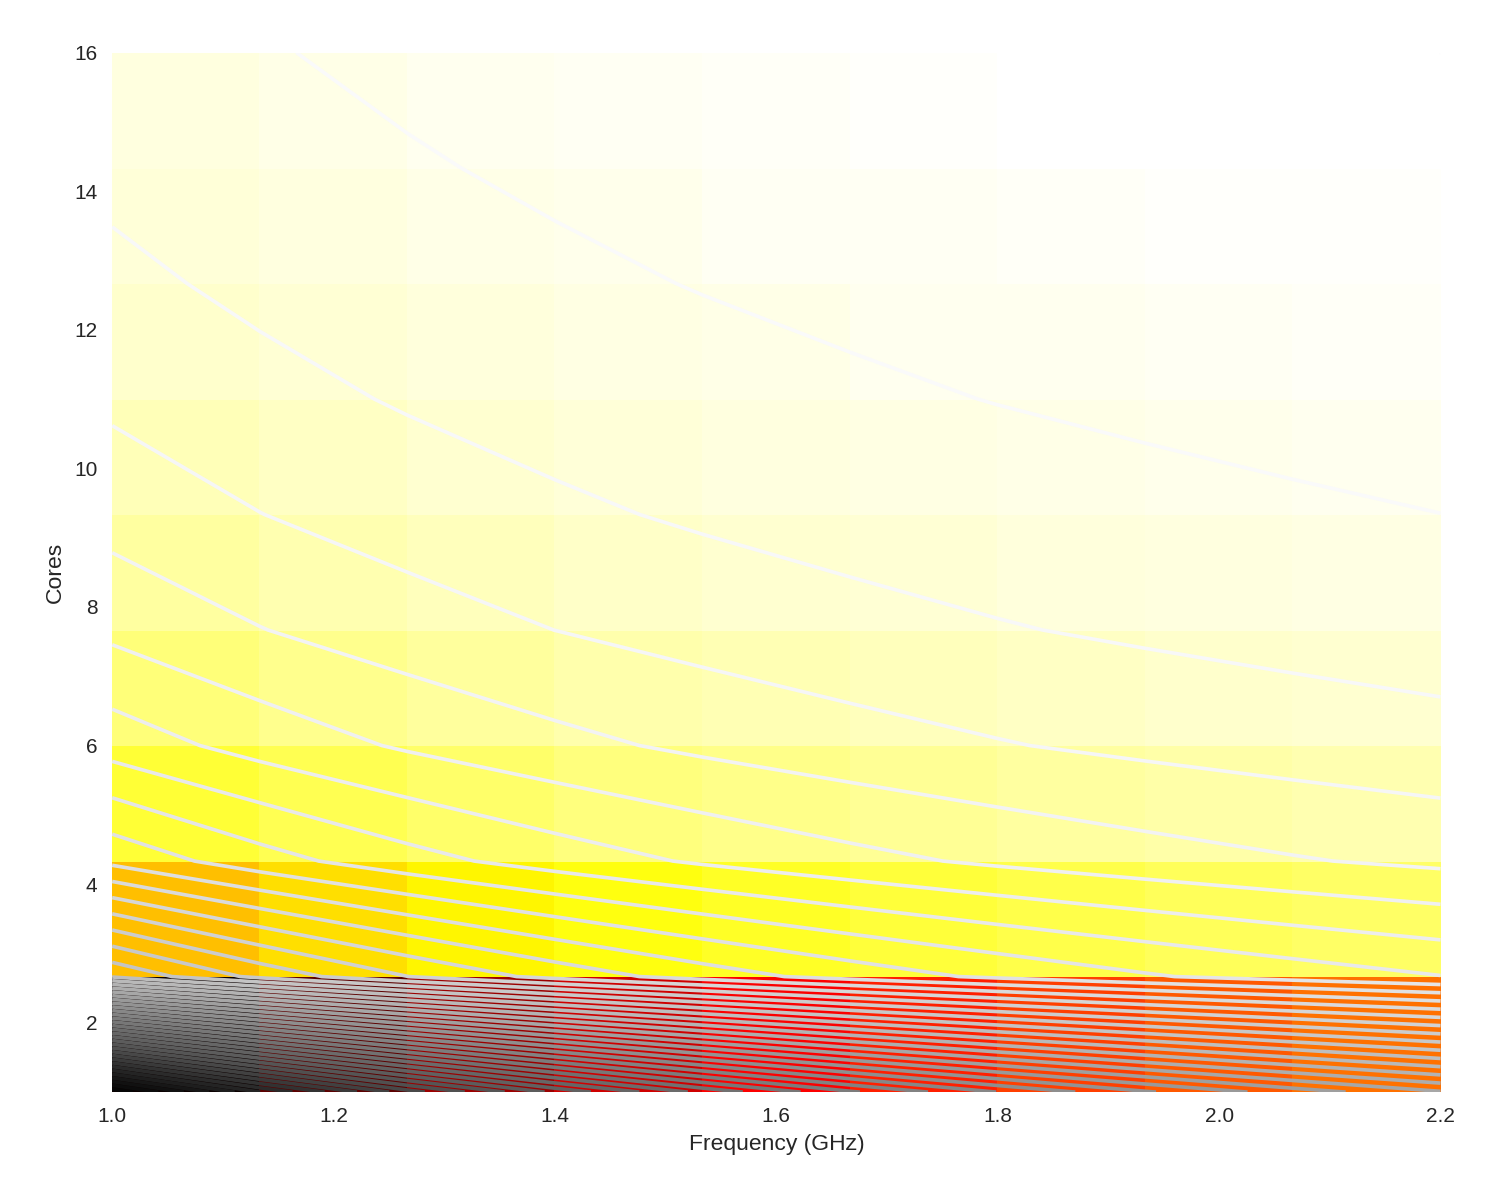
\includegraphics[width=\textwidth]{models/figures/analisys/w1.png}

	\end{subfigure}

	%

	\begin{subfigure}[b]{0.45\textwidth}

		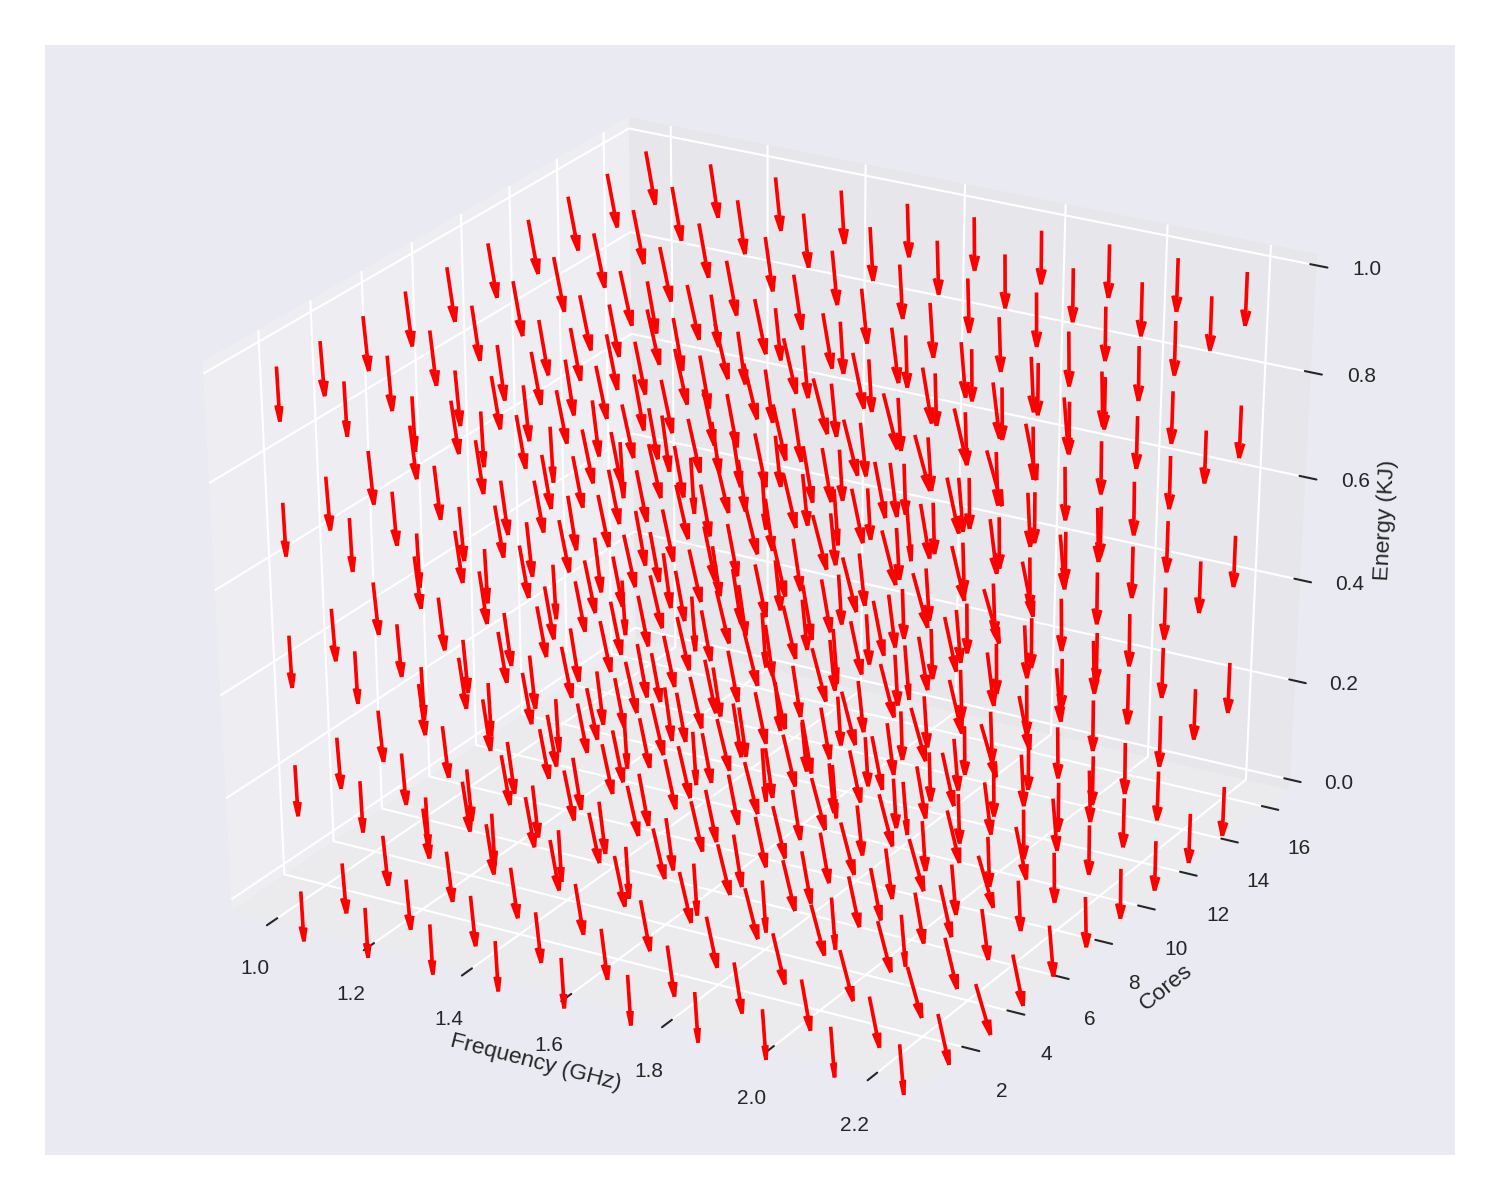
\includegraphics[width=\textwidth]{models/figures/analisys/w1_3d.png}

	\end{subfigure}

\end{figure}

